\documentclass[11pt,english]{report}

\usepackage{bussproofs}
\usepackage{minted}
\setminted{encoding=utf-8}
\usepackage{fontspec}
\setmainfont{FreeSerif}
\setmonofont{FreeMono}
\usepackage{tikz}
\usepackage{tkz-euclide}
\usetikzlibrary{automata,positioning}
\usepackage{amssymb,amsmath}
\usepackage[makeroom]{cancel}
\usepackage[left=2cm,right=2cm,top=2cm,bottom=2cm]{geometry}
\usepackage{multicol}
\usepackage{indentfirst}
\usepackage{unicode-math}
\usepackage{float}
\usepackage{subcaption}
\usepackage[backend=bibtex,style=numeric]{biblatex}
\bibliography{docs/report}
\usepackage{hyperref}
\hypersetup{
    colorlinks,
    citecolor=black,
    filecolor=black,
    linkcolor=black,
    urlcolor=black
}

\usepackage{pgfplots}
\usepgfplotslibrary{fillbetween}
\usetikzlibrary{plotmarks}

\newcommand{\getstat}[1]{docs/statistics/#1}

\newcommand{\vidpic}[1]{
	\includegraphics[scale=0.44]{docs/report/#1}
}

\newcommand{\statplot}[4]{
	\addplot[#3, mark = #4, thick, smooth, mark size = 2, mark options={fill=#3}] table [y=#2, col sep=comma] {\getstat{#1}};
}

\makeatletter
\renewcommand*\env@matrix[1][*\c@MaxMatrixCols c]{%
  \hskip -\arraycolsep
  \let\@ifnextchar\new@ifnextchar
  \array{#1}}
\makeatother

\newcommand*{\angleframe}[7]{%
\begin{scope}[xshift  =#4, yshift = #5,
			every node/.append style = {yslant = #7},
			yslant = #7,
			local bounding box = #2]
\node[#1] at (#6,#6) {};
\node[label, yslant = -#7, above right=9em and -0.75em of #2.south east](#2-label) {#3};
\end{scope}
}

\author{
	Aurimas Blažulionis (2069871)\\
	Alexander Krull\\
	\texttt{axb1440@student.bham.ac.uk}
}

\title{Optical Flow Processing Stack and Use of MPEG Motion Vectors}

\begin {document}
\maketitle

\section*{Abstract}

Tracking camera motion is an important task in many industries, including film, augmented reality and robotics. Detecting whenever there is motion in video is important for various other tasks, such as reducing the amount of storage used by CCTV cameras. In both of these cases, motion is extracted from video and is then processed. One, widely used method to describe motion is called optical flow. However, it is typically computationally expensive to calculate. MPEG's H.264 and other video compression standards coincidentally happen to encode motion in order to minimise new pixel data needed across consecutive frames. The aforementioned codec is often hardware accelerated on commodity hardware, meaning it could be possible to build an efficient optical flow pipeline and perform motion detection and tracking tasks at low cost. However, these optical flow fields are very noisy due to video encoders prioritising storage efficiency over motion accuracy. This project analyses how useful MPEG motion vectors are for motion detection and tracking tasks, compared to other industry standard methods, proposes a general framework for processing optical flow fields dubbed "OFPS", as well as an accompanying app that is able to perform motion detection and tracking tasks alongside a custom 3D renderer that is able to visualise tracking results.

\tableofcontents

\par\noindent\rule{\textwidth}{0.4pt}

\chapter{Introduction}

Camera motion estimation is a task of determining how a camera moves in 3D space over time. Film industry relies on this task being performed accurately in order to overlay computer generated imagery atop filmed video, augmented reality applications attempt to perform the same process, but in realtime, while robotics industry has given this task the name of "visual odometry", and plenty of research has been put in performing it accurately on a live robot, while also extending it to perform dense reconstruction, simultanious localisation and mapping.

Typically, it is done by extracting moving features across frames and using a sufficient number of them to solve parameters of some camera motion model (description of camera motion). Two classes of feature extraction methods emerge: feature tracking and optical flow based. Feature tracking sparsely picks out highly contrasting parts of a frame and follows them for as many frames as possible. Meanwhile, optical flow represents apparent motion of objects across 2 consecutive frames and it can either be sparse or dense. An optical flow field is effectively a list of point and vector pairs representing 2D motion at given pixel coordinates. The key difference between these 2 methods is that feature tracking can represent motion with less error across a sequence of frames, while optical flow typically has more information for 2 consecutive frames, at a loss of continuity. Given the sheer amount of pixels needed to be processed, feature extraction step is often more expensive than 3D motion estimation. For instance, MaskFlowNet\cite{zhao2020maskflownet}, a state of the art dense optical flow generation method takes upwards of 300 milliseconds to compute per frame on a laptop GPU, while VOLDOR\cite{voldor} visual odometry system takes just 100 milliseconds to consume the outputted optical flow field and produce accurate visual odometry data.

\begin{figure}[!ht]
	\centering
	\begin{subfigure}{180pt}
		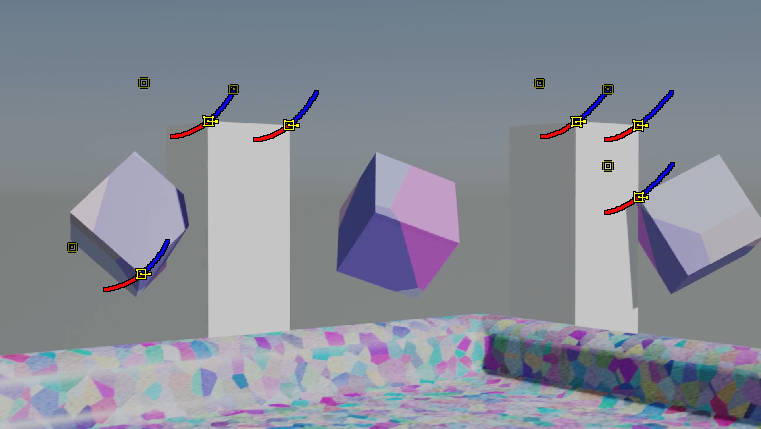
\includegraphics[width=180pt]{docs/report/feature-tracking.jpg}
		\caption{\centering Feature tracking.}
	\end{subfigure}
	\begin{subfigure}{180pt}
		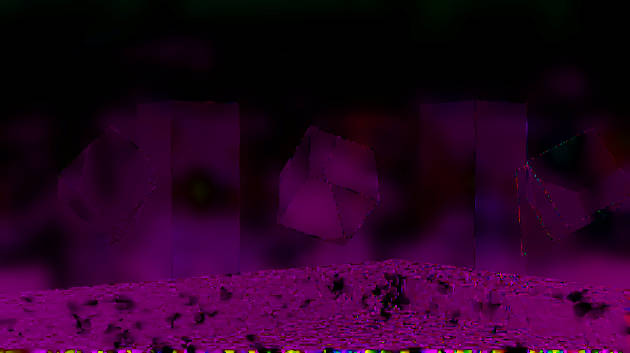
\includegraphics[width=180pt]{docs/report/optical-flow.jpg}
		\caption{\centering Optical flow.}
	\end{subfigure}
	\caption{\centering Feature tracking vs. Optical Flow. Tracking detects several key features and follows them over time, while optical flow aims to calculate direction vectors for a larger number of pixels.}
\end{figure}

Moving Picture Experts Group (MPEG) have designed a number of video encoding standards which heavily compress video files at low perceptual quality loss and they are ubiquitous to the point where most commodity hardware dedicate part of their silicon space for accelerated encoding and decoding of the latest MPEG video codecs - H.264/AVC\footnote{Advanced Video Coding}\cite{h264} and H.265/HEVC\cite{h265}. The way this compression works is that blocks of pixels get moved between frames in accordance to encoded motion vectors and only a small amount of new pixels are encoded to fill in the gaps and make small adjustments to the resulting frame. Essentially, to save space video encoding relies on apparent motion estimation, or in other words - optical flow field computation. Many hardware accelerated H.264 encoders are able to process over 30 frames per second at resolutions of 1080p, thus if one could extract the encoded motion in a H.264 stream, a highly efficient motion estimation pipeline could be built to produce 3D motion data in realtime. However, the primary task of a video encoder is to compress video, not to compute accurate optical flow, thus the resulting motion field is noisy\cite{1334181} (see figure 1.2) and not as dense as one would prefer. As a result, their usability for 3D motion estimation is uncertain.

\begin{figure}[!ht]
	\centering
	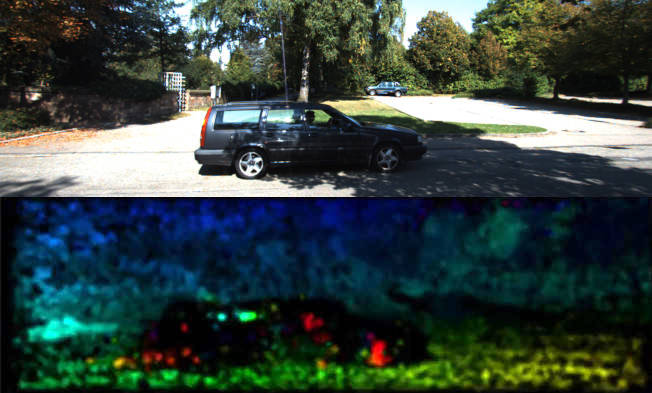
\includegraphics[width=190pt]{docs/report/mpeg-mvecs.jpg}
	\caption{\centering Still frame reference and optical flow from MPEG motion vectors.}
\end{figure}

This project analyses MPEG motion vectors, compares them against industry standard optical flow computation methods, looks at the ways they can be used in realtime operation and in the process we build a framework alongside an app for performing several motion processing tasks, such as motion detection and estimation.

\section{Project Aims}

The aim of this project is to build an integrated system for performing motion detection and camera tracking using high efficiency MPEG motion vectors. This project will focus on motion vectors created by H.264 video encoders, but will be built in a modular way so that different optical flow, motion detection and tracking methods could be composed. The motion tracking part of the project will be evaluated using synthetic 3D scenes, where precise camera motion is known. Quantitative results will be compared using different optical flow generation methods, as well as different motion tracking methods. The system will also be tested against several real world clips where a camera pans around a relatively stationary point. Evaluation against real-world clips will be less quantitative, but will focus more on whether it "looks good". Motion detection will be tested against a live H.264 stream coming from a Raspberry Pi, emulating CCTV camera conditions. The project aims to package this into a set of modular libraries and an application that provides a user-friendly interface for loading up pre-recorded or live videos and performing these motion detection and tracking tasks.

\section{Related Work}

There are several papers exploring motion tracking using MPEG motion vectors\cite{1334181}\cite{1414440}\cite{825867}. Another paper improves upon the previously mentioned techniques and achieves comparitavely high accuracy using simple motion field modeling and RANSAC for outlier removal\cite{almeida}. It is promising, however, due to its method not taking into account camera's field of view, the estimates of motion will only be correct up to a scale factor (thus their analysis only computed model's corellation not error). In addition, the authors' motion models are not accurate at the edges of the screen, thus there seems to be room for improvement (this point is related to not knowing the camera's field of view). Furthermore, the paper does not go into detail how exactly they implemented RANSAC - the inlier/outlier criteria is not specified. Overall, this paper is a good implementation candidate, but will require further development to complete it.

Broader, there is plenty of work in multiple view geometry. Several industry standard tools work on sequences of tracked 2D points, including Blender's\footnote{Open-source 3D modelling software.} libmv\cite{libmv} and OpenCV\cite{opencv5calib}. There also exists a paper improving the algorithms employed by the libraries, and works with just 5 data points\cite{1211470}. At the base case, the underlying algorithms attempt to estimate a matrix that relates points between images, known as fundamental matrix. There is an implicit problem of scale ambiguity\cite{hartley_zisserman_2004} with these methods - it is difficult to have consistent positional scale throughout time, because computed matrices produce translation values accurate only up to a scale factor. The aforementioned libraries have built-in algorithms for solving the problem for a sequence of frames, and they are proven to work well, but points need to be tracked throughout the sequence, which makes it unsuitable for optical flow.

There is recent work on creating visual odometry from dense optical flow fields\cite{voldor}, which is typically combined with a dense optical flow estimator, such as MaskFlowNet\cite{zhao2020maskflownet}. VOLDOR\cite{voldor} is a novel approach that models a probabilistic model of the optical flow field, iteratively estimates a depth map from a series of moving frames and outputs camera poses. Unfortunately, VOLDOR is not able to build a depth map with MPEG motion vectors due to their noisiness.

\begin{figure}[!ht]
	\centering
	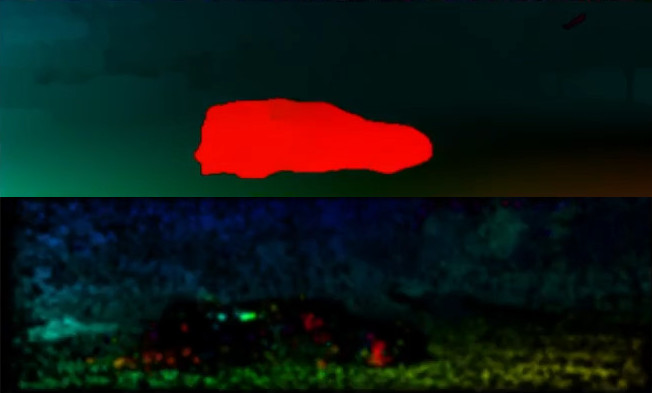
\includegraphics[width=190pt]{docs/report/mpeg-maskflownet.jpg}
	\caption{\centering MaskFlowNet (above) vs. MPEG (below).}
\end{figure}

Neither of the mentioned work solves the our problem completely. Thus, we believe there is a gap in current research and development, due to no system existing for doing realtime absolute motion tracking using MPEG. The papers either sacrifice realtime performance for accuracy, or are underspecified and too unconstrained. Other work does not suit optical flow very well, and by extension is not perfectly suitable for our domain. Thus, we will attempt to combine several of these methods, propose potential improvements and analyse what works best.

\chapter{Background}

This chapter introduces several concepts related to the project, most notably lower level details of MPEG compression, basics of epipolar geometry, and formal description of the problems we aim to solve.

\section{MPEG Video}

Motion Picture Experts Group has developed a number of video encoding standards over the years. The first one being MPEG-1 and was released in 1993. Fundamentally, it is very similar to currently one of the most widely used H.264/AVC/MPEG-4 Part 10 standard, which was published in 2004. This section will discuss features relevant to the project that exist in H.264 and older versions, but will not cover H.265, due to large differences in the standard.

\subsection{Encoding}

Various video streaming websites serve H.264 encoded video. YouTube recommends a 1080p video to be encoded at the bitrate of 8 megabits per second\cite{youtube}. For context, a single $1920 \times 1080$ RGB frame is nearly 8 megabytes of size, while a single JPEG will average between 100 and 300 kilobytes in size. For a 30 FPS video, YouTube asks each frame to average 34 kilobytes in size - that is $1/470$th of a raw frame, and around $1/5$th of a JPEG. Yet, a video with such high compression will look sufficiently high quality for a viewer not to notice any artifacts. The reason this is possible is due to intra-frame compression.

An MPEG video consists of several sparsely placed intra-frames, known as \textbf{I-frames} and series of predicted frames (\textbf{P-frames} and \textbf{B-frames}). Intra-frame is effectively a JPEG image, while a predicted frame contains changes in relation to other frames. The difference between P and B frames is that P frames only look at a keyframe behind (I or P frame), while B frames are interpolated bi-directionally between the previous and the next keyframes. A single intra-frame and all subsequent predicted frames form a group of pictures, known as GoP.

\begin{figure}[!ht]
	\centering
	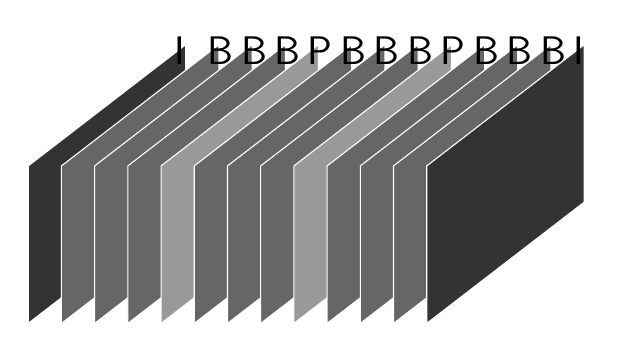
\begin{tikzpicture}
		\tikzset{
			basefont/.style = {font = \Large\sffamily},
			timing/.style = {basefont, sloped,above,},
			label/.style = {basefont, align = left},
			angleframe/.style = {basefont, white, align = center, minimum size = 2cm, fill = black!60, draw = white},
			iframe/.style = {angleframe, fill = black!80},
			pframe/.style = {angleframe, fill = black!40},
			bframe/.style = {angleframe, fill = black!60},
		};

		\angleframe{iframe}{frame1}{I}{0}{0}{1cm}{0.77}
		\angleframe{bframe}{frame2}{B}{12}{0}{1cm}{0.77}
		\angleframe{bframe}{frame2}{B}{24}{0}{1cm}{0.77}
		\angleframe{bframe}{frame2}{B}{36}{0}{1cm}{0.77}
		\angleframe{pframe}{frame3}{P}{48}{0}{1cm}{0.77}
		\angleframe{bframe}{frame2}{B}{60}{0}{1cm}{0.77}
		\angleframe{bframe}{frame2}{B}{72}{0}{1cm}{0.77}
		\angleframe{bframe}{frame2}{B}{84}{0}{1cm}{0.77}
		\angleframe{pframe}{frame3}{P}{96}{0}{1cm}{0.77}
		\angleframe{bframe}{frame2}{B}{108}{0}{1cm}{0.77}
		\angleframe{bframe}{frame2}{B}{120}{0}{1cm}{0.77}
		\angleframe{bframe}{frame2}{B}{132}{0}{1cm}{0.77}
		\angleframe{iframe}{frame1}{I}{144}{0}{1cm}{0.77}
	\end{tikzpicture}
	\caption{\centering A GoP of size 12. The ending I-frame starts the next GoP.}
\end{figure}

Predicted frames is how MPEG video is able to achieve such a high compression ratio. In AVC, each frame contains a number of transform and prediction macroblocks. Transform blocks are $4 \times 4$ or $8 \times 8$ sized chunks that describe new pixel values at part of the frame in a way where chroma values are subsampled to save space. Prediction blocks are $4 \times 4$ to $16 \times 16$ pixel sized chunks that get shifted across frames and motion of each macroblock is defined by a motion vector $\overrightarrow{v}$ - pixel data is reused and only moved from one location to the next. The motion of prediction blocks will be needed by the project and an extraction module will be built.

\subsubsection{"Datamoshing"}

An interesting experiment can be done to visualise how MPEG works by intentionally corrupting the encoded stream. In non-scientific literature this process is known as datamoshing. If a video contains just a single GoP, it is possible to replace the only I-frame in the video with a different image and visualy see what changes are encoded in the predicted frames throughout the entire clip. Most notably, high contrast areas are likely to be moved in accordance to camera motion, while low contrast areas are likely to blur themselves out due to the noisiness of the encoded motion vectors (see figure 2.1).

\begin{figure}[!ht]
	\centering
	\begin{subfigure}{230pt}
		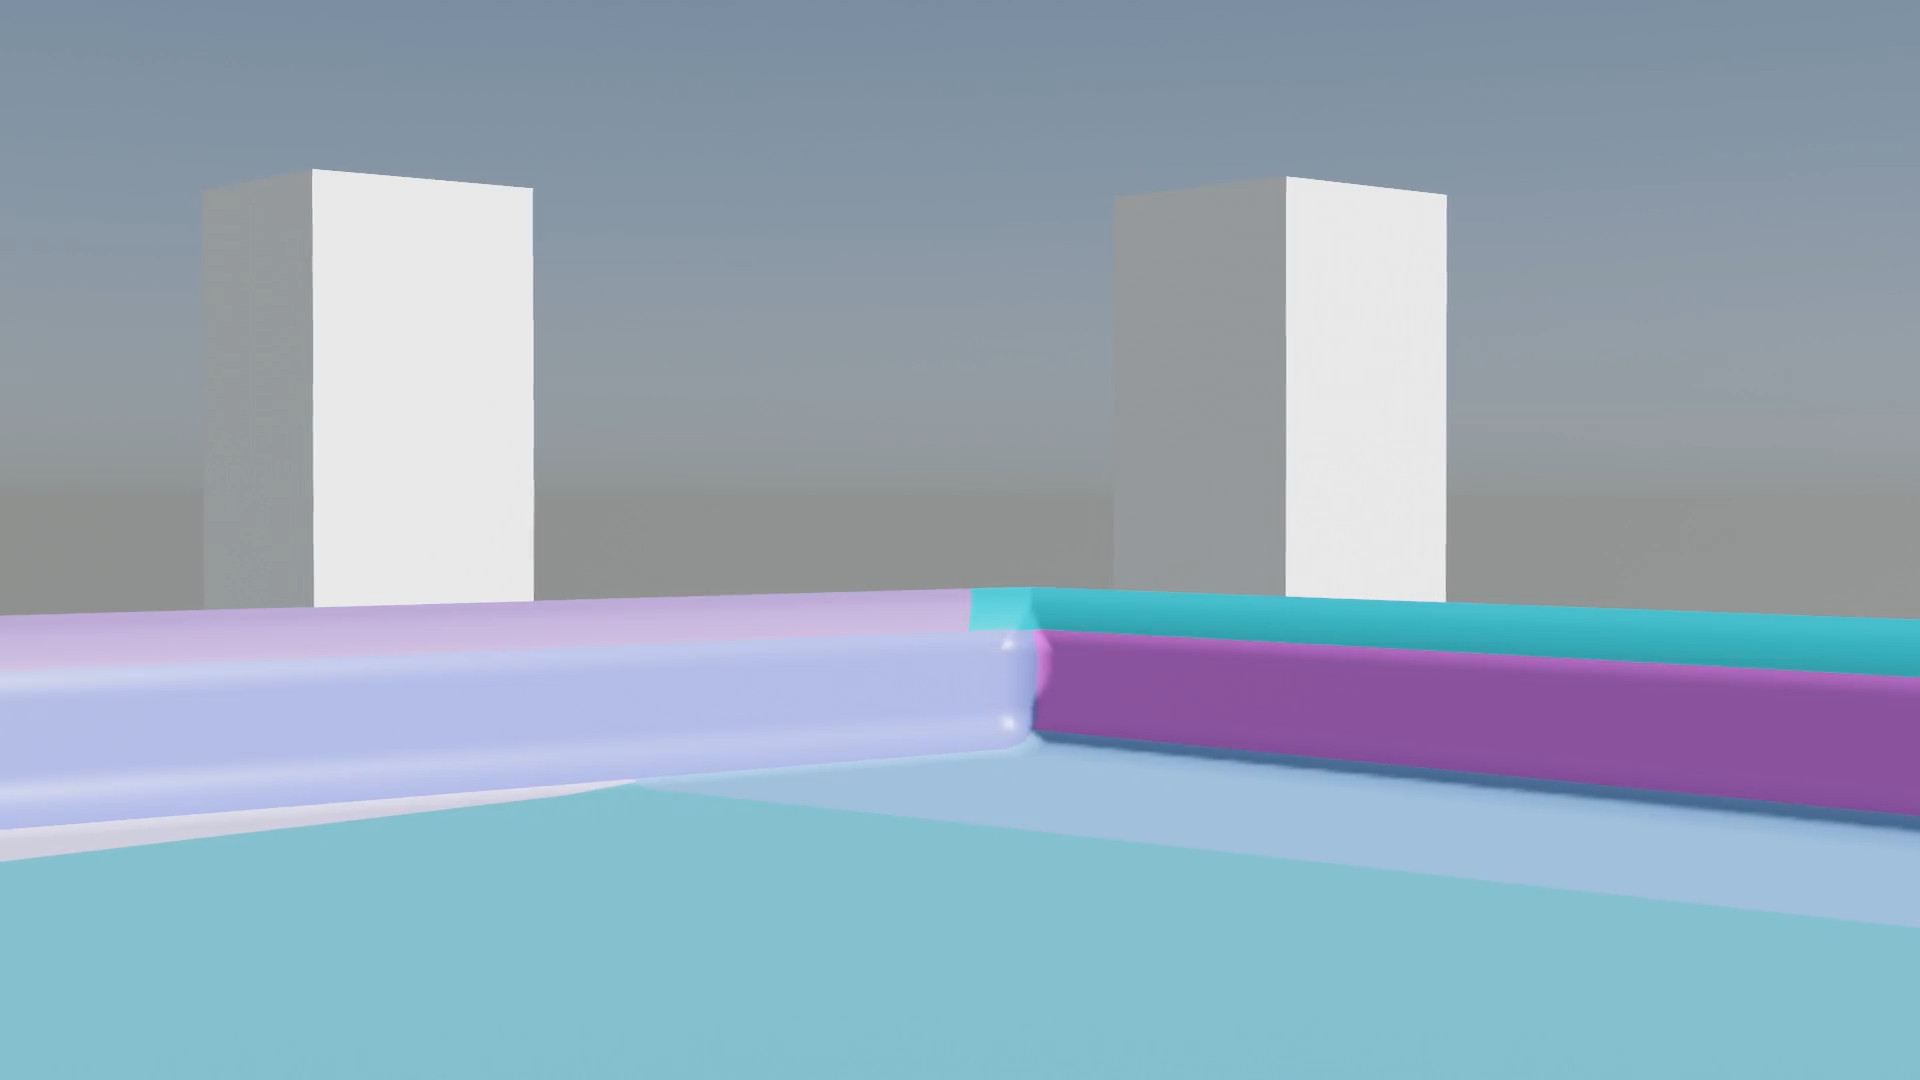
\includegraphics[width=230pt]{docs/report/mosh-original.jpg}
		\caption{\centering Original video.}
	\end{subfigure}
	\begin{subfigure}{230pt}
		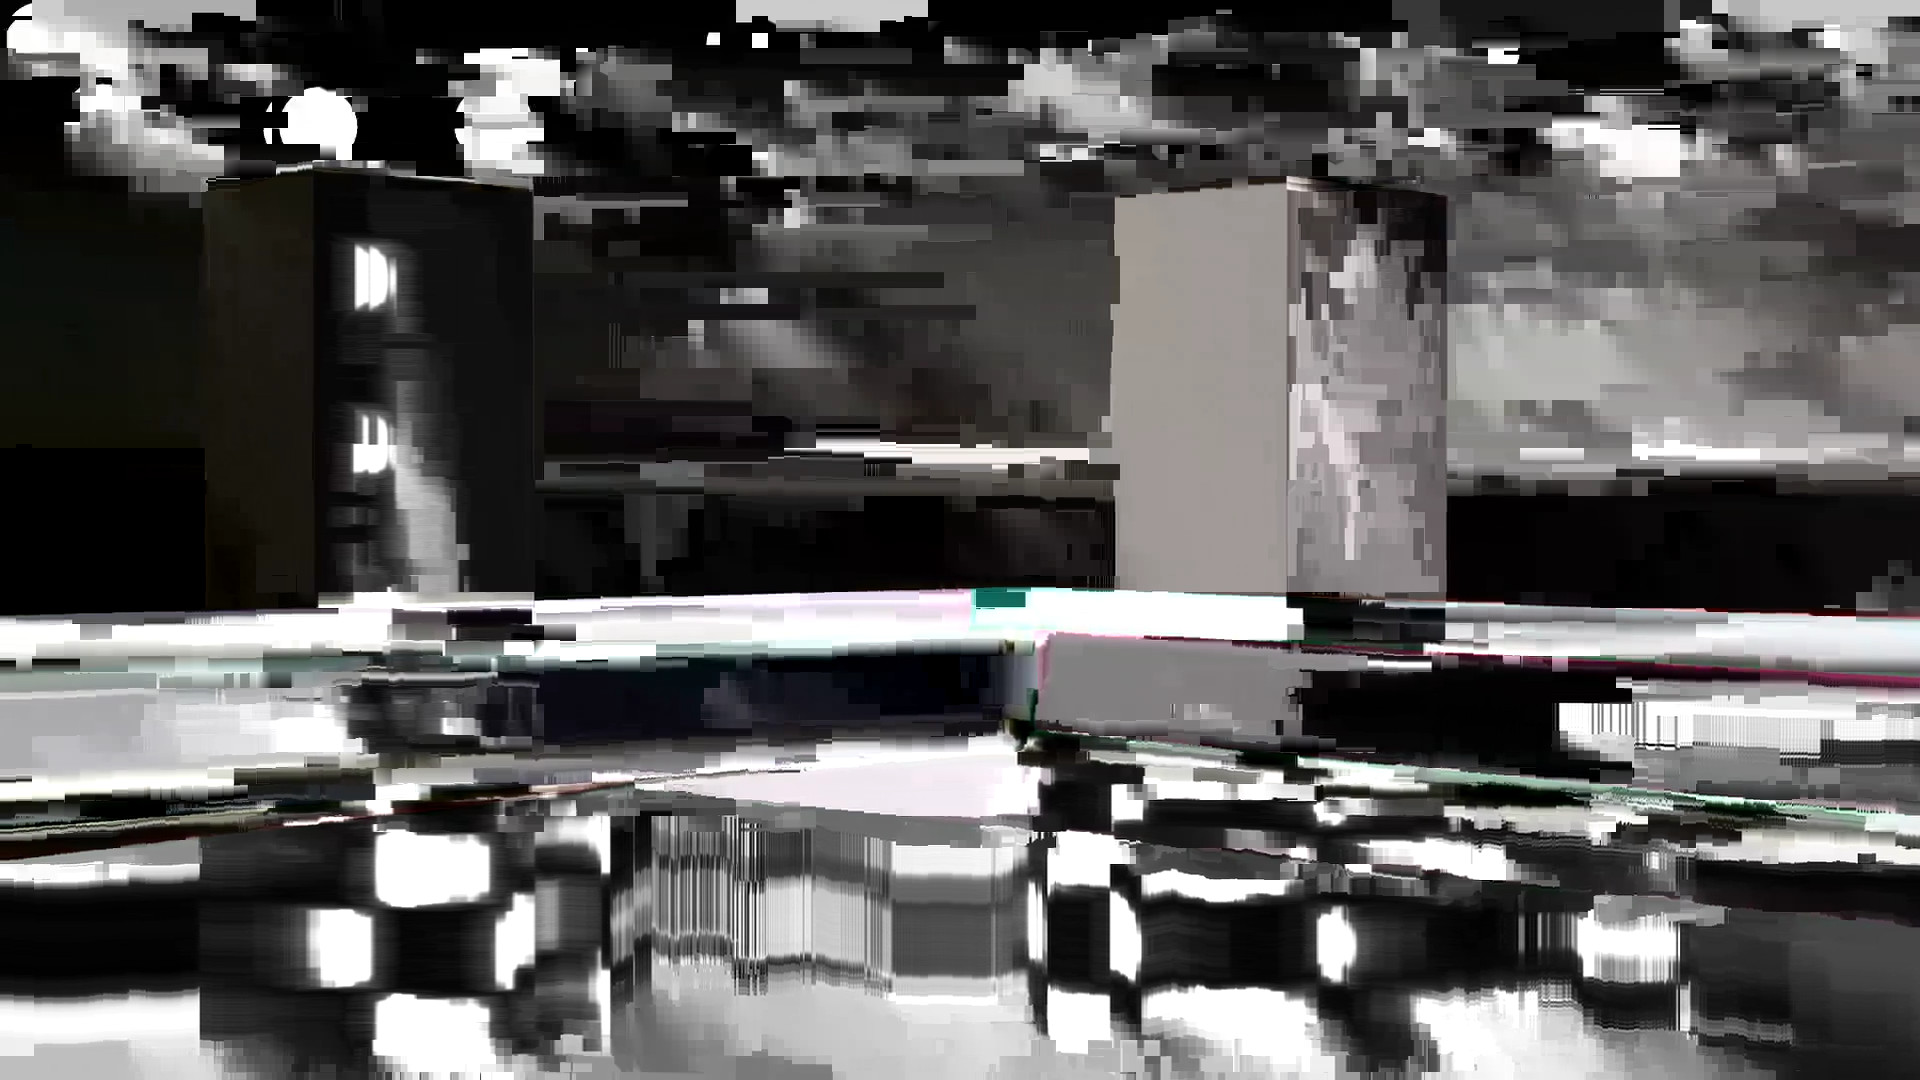
\includegraphics[width=230pt]{docs/report/moshed.jpg}
		\caption{\centering Video after datamoshing.}
	\end{subfigure}
	\begin{subfigure}{230pt}
		
\includegraphics[width=230pt]{docs/report/mosh-to.jpg}
		\caption{\centering Image the video was moshed with.}
	\end{subfigure}
	\caption{\centering Result of datamoshing. This is a single frame taken after several panning motions. The results can be reproduced using the provided script in the project's repository. Run scripts/mosh.sh and pass input video file together with image to mosh into the video. The script only supports 1080p video.}
\end{figure}

\section{Pinhole camera model}

The pinhole camera model is the simplest mathematical description of coordinate relationship in 3D space to their projection onto image plane of a camera. In this model, camera's aperature is described as a point, there are no lenses, and by extension - image distortion. Pinhole camera has a focal length $f$ that describes distance of the image plane to the aperature. Given a 2D point $p = (x, y)$, its projection on 1D image line will be on point $p_1 = -y * \frac{f}{x}$. The same concept extends to 3D space, except the points are projected onto 2D plane.

\begin{figure}[!ht]
	\centering
	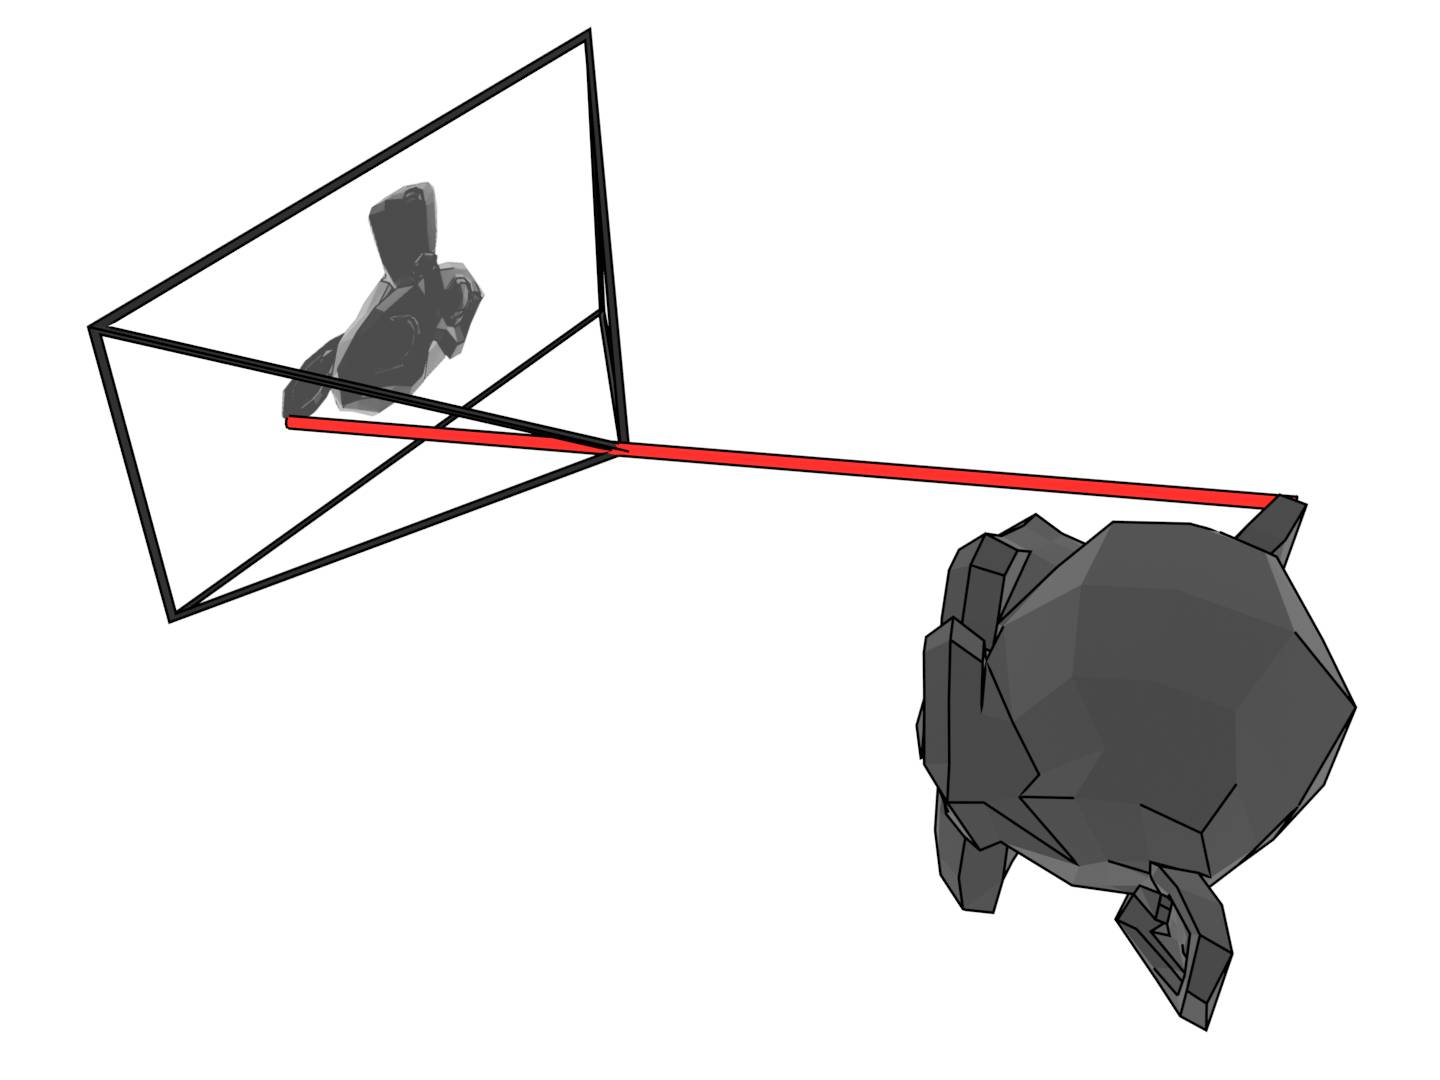
\includegraphics[width=270pt]{docs/report/pinhole-camera.jpg}
	\caption{\centering Geometry of a pinhole camera. All projections are originally upside down, but they get flipped in post-processing.}
\end{figure}

\section{Two-View Geometry}

Two-view geometry, also known as epipolar geometry concerns itself about the relationship of 2 views given 2D point correspondances. From a single view it is impossible to determine how far away a point in the image is - it only defines a line. In fact, a common way to look at pixels in computer vision is in terms of homogeneous coordinates - point $p = (x, y)$ can be represented as $l = (kx, ky, k)$.

Given a first view point $l = (kx, ky, k)$ in homogeneous coordinates, its correspondance in the second view $l' = (kx', ky', k)$, and relative pose between the views, these points can be intersected and a point in 3D space may be resolved. However, often times, pose of the views is unknown. Thus, to perform triangulation, relationship between the 2 views needs to be calculated from a number of 2D point correspondances in the form of a fundamental matrix.

\begin{figure}[!ht]
	\centering
	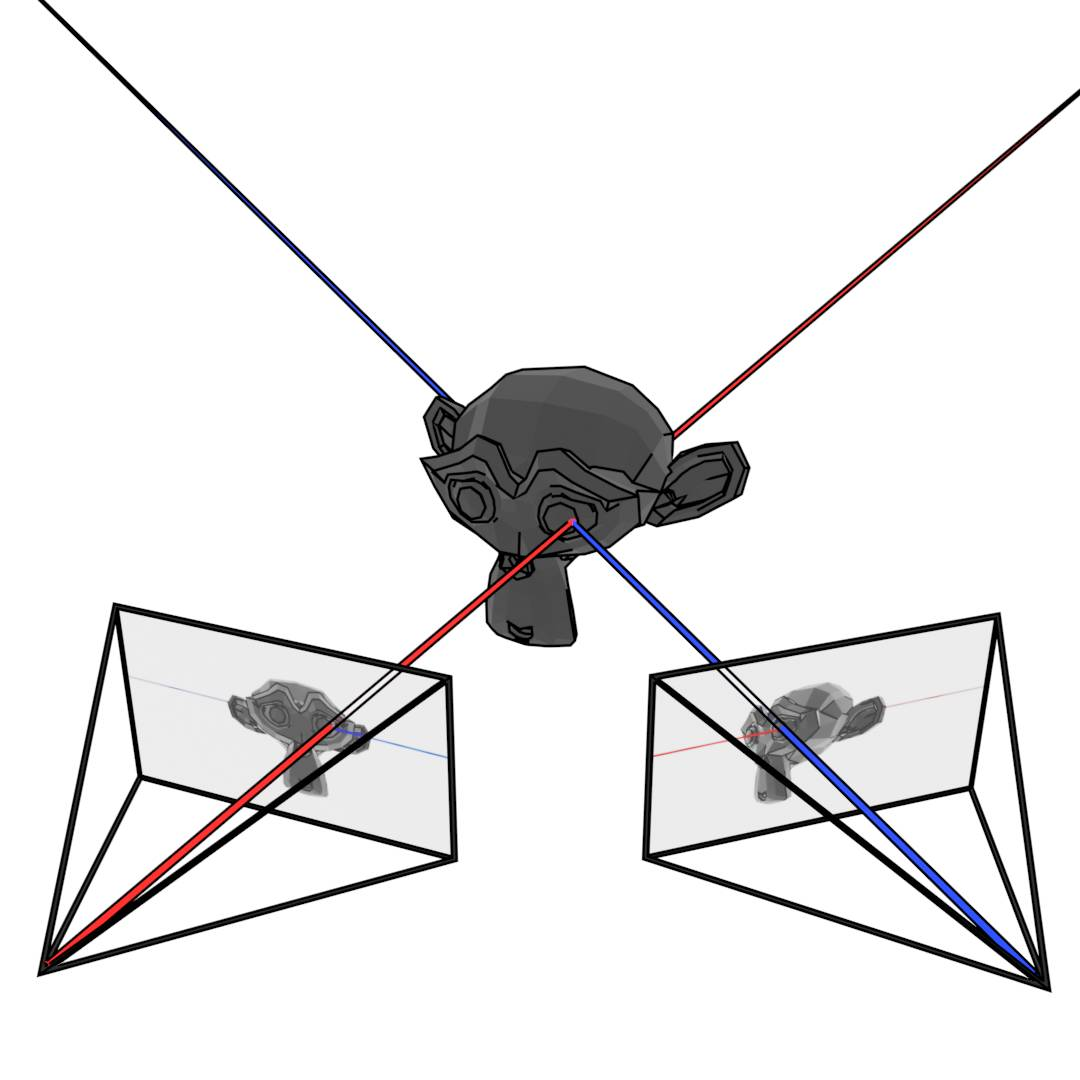
\includegraphics[width=270pt]{docs/report/epipolar-geometry.jpg}
	\caption{\centering Two-view geometry. Epipolar lines can be seen across the views, and they intersect in 3D space.}
\end{figure}

\subsection{The fundamental matrix}

The fundamental matrix is an algebraic representation of epipolar geometry. It is a $3 \times 3$ matrix of rank 2. If a point in 3-space $X$ is imaged as $x$ in the first view (in homogeneous coordinates), and $x'$ in the second, then the image points satisfy the relation $x'^T F x = 0$\cite{hartley_zisserman_2004}, i.e. $Fx$ becomes perpendicular to $x'$. The fundamental matrix has 7 degrees of freedom - it depends on both view pose changes, and intrinsic camera parameters. Several industry standard libraries implement algorithms for robust fundamental matrix estimation, such as Blender's libmv and OpenCV. There is a recent paper describing robust estimation from only 5 data points\cite{8578130}. Once a fundamental matrix is known, and given intrinsic camera parameters, it is possible to compute 3D positions of the 2D point correspondances, through the process of triangulation.

\subsection{The essential matrix}

If camera intrinsics are known (camera is calibrated), it is possible to use them to constrain the freedom of the fundamental matrix, and compute it more accurately, with fewer data points. The essential matrix is the the specialisation of the fundamental matrix to the case of normalised image coordinates\cite{hartley_zisserman_2004}. The essential matrix has fewer degrees of freedom - only 5. Other parameters are constrained by requiring knowlege of intrinsic camera parameters. OpenCV has an implementation solving the essential matrix using D. Nister's efficient 5 point algorithm\cite{1211470}. We will rely on both of these matrices when constructing some of our motion estimators.

\section{Problem formulation}

Having introduced background concepts, let us now formally define the problems we want to solve.

\subsection{Motion detection}

Given a list of motion vectors for a frame we want to determine whether the frame contains motion or not. That is, we want to build a function $f(V) = m$ that takes in motion vectors $V = \{(p_0, \overrightarrow{v_0}), (p_1, \overrightarrow{v_1}, \cdots, (p_n, \overrightarrow{v_n}))\}$ and produces boolean value $m$ indicating whether there is motion or not.

\subsubsection{Hypothesis}

We believe that it is possible to detect motion effectively using optical flow methods, and in particular, MPEG motion vectors.

\subsection{Motion estimation}

Given a list of motion vectors for a frame we want to estimate camera's movement in 3D space. That is, we want to build a function $f(V, K) = (\overrightarrow{t}, q)$ that takes in motion vectors $V = \{(p_0, \overrightarrow{v_0}), (p_1, \overrightarrow{v_1}), \cdots, (p_n, \overrightarrow{v_n})\}$ together with camera intrinsic matrix $K$ and produces translation vector $\overrightarrow{t}$, as well as rotation quaternion $q$ that both describe change of camera's pose in relation to the previous pose.

\subsubsection{Hypothesis}

We hypothesise that camera motion estimation may be possible with optical flow methods, in particular - MPEG motion vectors. We want to track all 6 degrees of freedom. However, if this hypothesis turns out to be incorrect, our second hypothesis is that resolving just the camera's orientation $q$ may still be feasible.

\chapter{Methods and Implementation}

This project contains a lot of moving parts across different disciplines: setting up hardware, software architecture design and development, paper implementation and improvements. Initially, the project focused around motion vector extraction from H.264 streams and involved testing its functionality. Later, it built several 3D motion estimation modules, starting from Almeida, then attempting to use libmv and OpenCV. Due to imperfect results, a different optical flow processing task was found - motion detection and thus a module was built for that purpose. Finally, once the library and accompanying modules proved to work sufficiently well, the core API was reworked, dynamic loading was built-in and a user friendly application was designed, which required further development, such as a 3D renderer, to present the results intuitively. The sections below describe the progress in the previously given order.

Most of the code was written in Rust. It is a systems programming language that maximises performance without sacroficing safety, language abstractions and modularity. Given the project is focused around performance, the language was a clear choice. Standard Rust toolchain is employed, the current compiler version being 1.59.0. The project is compiled using standard cargo utility. The only non-standard part is the libmv module and its nuances will be explained in the dedicated section.

\section{Optical Flow Processing Stack}

OFPS is the core library of the project. It contains everything needed for the user to process optical flow. Primary focus was developing an architecture that was both trivial to use and could scale well, i.e. able to support any future methods of motion extraction, detection and estimation. Thus, the library did undergo iterative development with small changes to the API as time passed. Nalgebra was chosen as the primary numpy-like math crate\footnote{Library in Rust terms} due to its flexibility, ease of use and proven time record.

\subsection{Pinhole camera}

We define a standard pinhole camera model. The key design decision was to make resolution information unnecessary when processing optical flow, thus pixel coordinates are normalised in $[0; 1]$ range and the principal point\footnote{Point of the aperature} is at $(0.5; 0.5)$. Effectively all images are stretched to have square aspect ratio. This is a similar concept to anamorphic lenses - film industry often uses special lenses that have a higher horizontal field of view by bending the incoming light more horizontally than vertically. The frame then needs to be stretched out in post-production. Our pinhole camera model essentially does the same - vertical and horizontal fields of view are independent, which is equivalent to having differing focal lengths. Any processing algorithm then uses these intrinsic parameters instead of video resolution to process the motion vectors.

\subsection{Interface design}

Three generic interfaces, known as traits in Rust, were developed to provide a simple yet flexible standard for motion decoding, estimation and detection. In addition, one general interface for configuring underlying properties of the plugins was defined.

\subsubsection{Decoder}

A Decoder either extracts precomputed motion from an input stream, or calculates it from image data. The input stream is not visible to the user - it is stored within the decoder. Initially, Decoder was designed to output a MotionField, which is a dense fixed-size optical flow structure. Producing fixed-size fields may result in predictable performance characteristics, however, it was noticed that sampling raw motion vectors into fixed resolution structure lowered accuracy of the estimators consuming the fields, thus the motion is now being outputted as a list of motion vectors - pairs of points representing the location of motion on screen and vectors representing the motion. To make code resolution-independent, screen locations and motion vectors are normalised in $[0; 1]$ range. The interface was designed to support cases with no motion information present (e.g. I-frames) and it supports optional output of RGB frames. It is optional due to some decoders potentially not having any access to raw frame data, e.g. precomputed motion fields and specialised video decoders that only extract motion vectors. There are also several optional fields to provide timing and video aspect ratio information. Overall, the trait does not impose any unnecessary requirements that would lower performance of the decoding.

\subsubsection{Estimator}

An Estimator accepts a list of normalised motion vectors alongside pinhole camera and outputs estimated rotation and translation of the camera. The estimator is responsible resolving translation scale ambiguity and thus is not guaranteed to be stateless - motion estimator may rely on previous inputs to produce more accurate estimates of transformation.

\subsubsection{Detector}

A Detector takes a list of normalised motion vectors and outputs whether there is motion or not. It is optionally able to return a dense motion field describing the motion, if there is any, however, it is not a required functionality.

\subsubsection{Properties}

Properties trait is implemented by all plugins. It is a trait that provides a list of string, boolean, floating point and integer properties that are available to be configured when using arbitrary decoder, estimator or detector. This trait is useful when paired with the plugin system, and is used by the OFPS Suite application to provide further user control.

\subsection{Plugin System}

To make the stack modular we added dynamically loadable plugin system. A PluginStore object searches the current working directory, executable's directory, and several other predefined directories for shared libraries that implement OFPS traits. All discovered libraries are stored and get loaded upon request. define\_descriptor macro is used by each library to define which OFPS traits are implemented. A special header gets created that then gets parsed by OFPS plugin loader. It contains the name of the plugin, initialisation function and several safety fields.

We had to add certain restrictions to ensure safety when loading these plugins. Since Rust is an evolving language, it does not yet define a stable Application Binary Interface (ABI)\cite{abi-ip} and code compiled on different compilers may be incompatible in subtle ways. This can lead to runtime crashes, or worse, unintended changes in program's control flow. One way to approach this problem would be to utilise CGlue opaque objects\cite{cglue}, which are essentially thinly wrapped objects in stable C ABI. It would provide the most safety possible, however, nalgebra and other extensively used crates use C-incompatible structures, and would require to be converted to C-compatible types when passing interface boundaries. Imposing such requirements would make OFPS too verbose to use and thus an alternative approach was taken. For the following approach we rely on present-day fact that language ABI can only change either when compiler gets updated, or when a special unstable -Z randomize-layout\cite{randomize-layout} flag is used. Concluding that on stable Rust toolchain ABI never changes, we added compiler version checking to the plugin loader. In addition, a special API\_VERSION constant was added to prevent loading API-incompatible code. In the end, we get a stable and modular dynamically loadable plugin system in a programming language that does not provide such facilities.

\section{Raspberry Pi setup}

A 8GB Raspberry Pi 4 was acquired with a OV5647 camera sensor for the purposes of live project testing. Standard Raspberry Pi OS was installed and only video RAM was increased. The onboard Broadcom BCM2711 system-on-chip contains a H.264 hardware encoder, capable of processing 1080p frames at 30 frames per second. A script was set up to start a program that encodes live video from the camera and outputs resulting packets to a remote client through a TCP server that is accessible on local network. To increase the number of P-frames we customise the GoP size to 240 frames, meaning there is typically just a single I-frame every 8 seconds.

\section{Optical flow field decoders}

Several optical flow generation methods were developed. They are split into separate crates and each provides an object that implements the Decoder trait. These crates can be compiled independently into shared libraries that are loadable by OFPS plugin system. This section describes each of the built-in decoders.

\subsection{AV}

AV decoder has its crate named mvec-av, and is responsible for decoding motion vectors using LibAV and FFMPEG. It supports H.264 decoding and extraction of motion vectors. Several container types are supported, such as MKV, MP4, and MOV. We had to set up a custom input stream for LibAV to be able to process any Rust byte stream. The library always performs full H.264 decoding, thus performance may not be optimal for our case. A way to solve this would be to patch libav to only output motion vectors\cite{libav-patch}, but that would require non-standard build procedures. On the other hand, results will show that it still is sufficiently performant.

\subsection{OpenCV}

OpenCV decoder has its crate named mvec-cv, and is responsible for computing optical flow using either Gunnar-Farneback algorithm\cite{Farnebck2003TwoFrameME} or RLOF\footnote{Robust Local Optical Flow}\cite{rlof}. The computed flow is then outputted to the user.

\subsubsection{Gunnar-Farneback}

Gunnar-Farneback algorithm calculates a semi-dense optical flow, meaning most of the pixels contain motion information. If the area is of very low contrast, or there is no motion, that pixel will have have motion value equal to $\overrightarrow{0}$. Thus, there is a trade-off between returning all zero vectors, which could potentially skew the results in motion, or no zero vectors, which could skew the results when there is no camera motion. To solve this, a mask is applied to only output motion vectors in high contrast areas. The mask is computed by using sobel filter that is then thresholded and dilated. This proved to work well in both cases.

\begin{figure}[!ht]
	\centering
	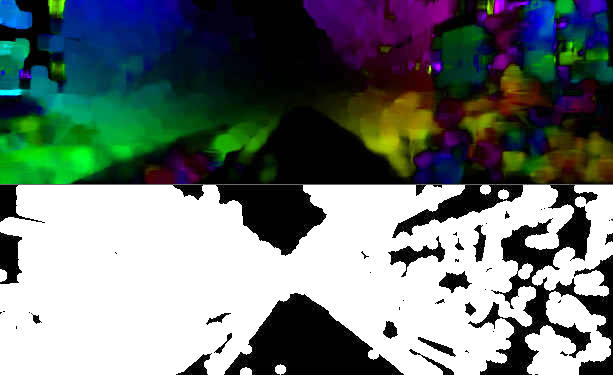
\includegraphics[width=190pt]{docs/report/gunnar-farneback-mask.jpg}
	\caption{\centering Example of contrast mask built for Gunnar-Farneback post-processing (below), next to optical flow produced by the algorithm.}
\end{figure}

\subsubsection{RLOF}

Robust Local Optical Flow is a newer optical flow computation method. We implemented it, because while Gunnar-Farneback is way more documented, RLOF appears to be more accurate then Gunnar-Farneback's algorithm. This algorithm can be toggled through the properties system.

\begin{figure}[!ht]
	\centering
	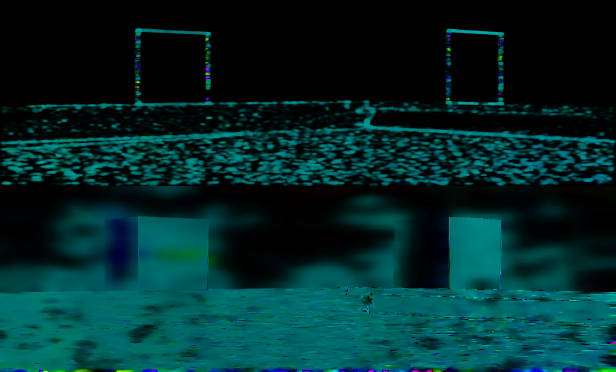
\includegraphics[width=190pt]{docs/report/farneback-vs-rlof.jpg}
	\caption{\centering Farneback (above) method vs. RLOF (below) in the context of camera panning right.}
\end{figure}

\subsubsection{Downsampling}

High resolution dense optical flows are computationally expensive to process by motion estimators, thus it was desirable for us to produce lower resolution flows. However, as part of our testing we noticed that low resolution image inputs lead to very low quality optical flows. Thus, we added an option to calculate optical flow using input image resolution, and then downsample it to lower resolution output.

\section{Motion estimation}

Several 3D motion estimation modules were developed. They are split into separate crates and each of them contains a structure that implements the Estimator trait. This section describes the details of every estimator individually.

\subsection{Modified Almeida estimator}

We implement the method proposed by Almeida et al. that finds the best-fit affine model to estimate camera motion by using least squares method\cite{almeida}. The crate of the implementation was named almeida-estimator. We modify their paper to suit it to our problem and to introduce several improvements to the algorithm. This method only produces rotation and zoom information - no 3D position changes. Since the Estimator trait requires prior knowlege of camera intrinsics, we will remove computation of lens zoom. However, Estimator's rotation output must be absolute and the proposed algorithm does not produce such values. We solve this issue by modeling our own panning, tilting and rolling prototypes, that are computed using camera intrinsics. The prototypes are essentially discrete derivatives of rotation by some angle $\epsilon$, and in the implementation it was set to 0.1 degrees.

\subsubsection{RANSAC}

Authors used RANSAC\cite{FISCHLER1987726} (RANdom SAmple Consensus) algorithm to make estimations more robust by filtering outliers. The algorithm computes model parameters from a minimal subset of randomly picked data samples and then compares how well the model fits other samples. The samples that the model fits well are called inliers. The process repeats for a number of iterations and the model with the largest inlier set is returned.

The metric used to check whether a sample is an inlier or not depends on the problem being solved and the paper does not specify it. In simple problems, such as line fitting, euclidean distance is often used as an evaluation metric. Given a point $p$ and its estimate $h$, checking if the point is an inlier can be done by checking whether $||p - h|| \leq c$ holds true, where $c$ is a constant threshold. Due to projective distortion, this does not work for our problem. With wide camera view, apparent motion at the center of the frame does not match the motion at the edges of the screen - the latter points have bigger apparent motion than ones at the center. Thus, we had to develop our own metric that works sufficiently well for our problem.

Given a pixel in the view at angle $\alpha$ from the center of view, rotating the camera towards that point by small angle $\theta$ will produce apparent motion that is higher than the motion at the center of view by the factor of $\frac{1}{cos(\alpha)}$. Thus, given a point at angle $\alpha$, its motion vector $\overrightarrow{v}$, model estimate $\overrightarrow{h}$ and theshold $c$, determening whether a sample is an inlier or an outlier can be done by checking whether $||\overrightarrow{h} - \overrightarrow{v}|| * cos(\alpha) \leq c$ holds true. However, vertical and horizontal angles can differ significantly, which could lead to high tolerances for error in non-dominant motion, thus our implementation computes 2 different angles $\alpha_x$ and $\alpha_y$ for horizontal and vertical axis respectively. Afterwards, $||(cos(\alpha_x) (h_x - v_x); cos(\alpha_y) (h_y - v_y))|| \leq c$ is used to determine whether the inlier status of the data sample.

\begin{figure}[!ht]
	\centering
	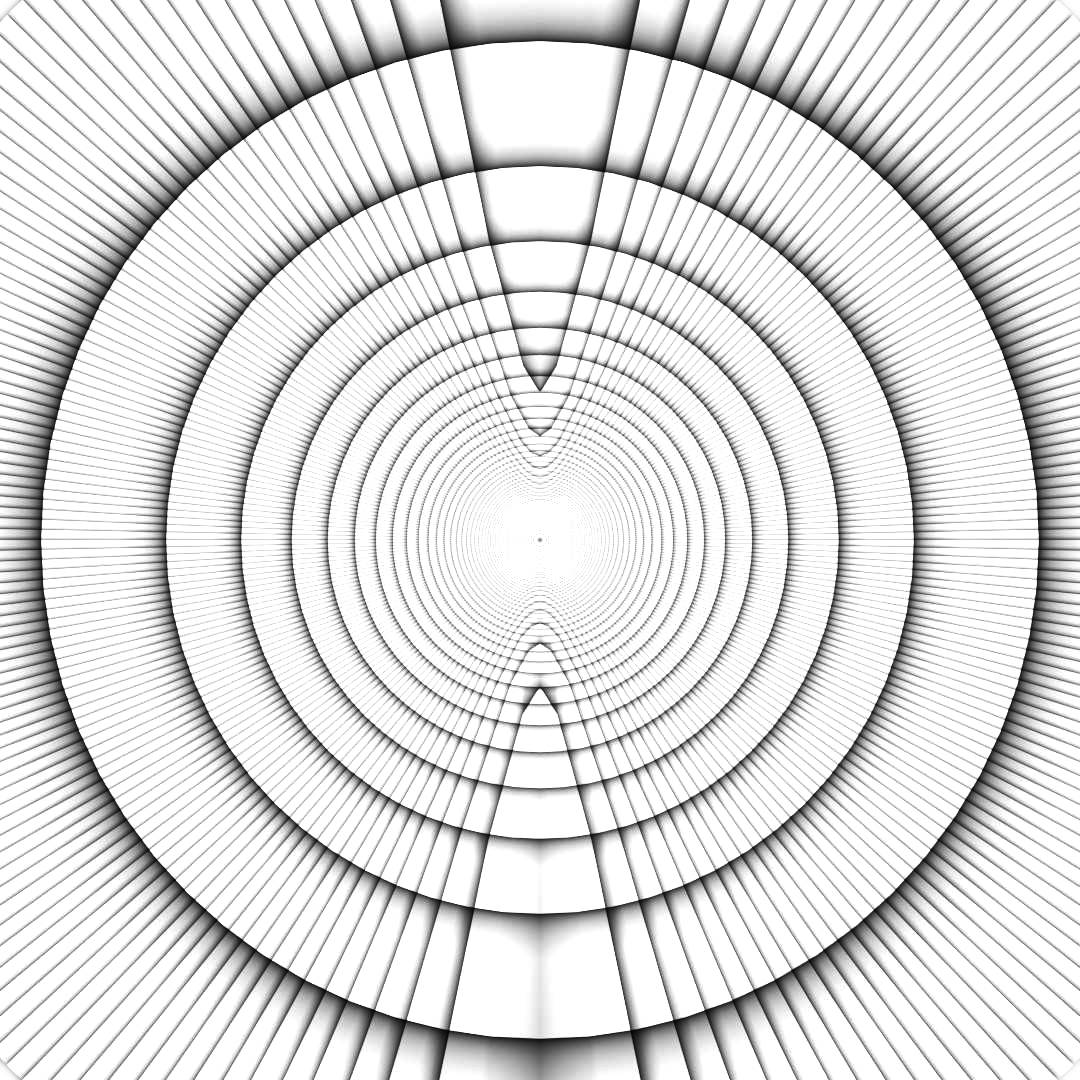
\includegraphics[width=150pt]{docs/report/distortion.jpg}
	\caption{\centering Projective distortion. All lines are drawn on a sphere at identical angle intervals. Camera's field of view is close to 180 degrees. Lowering the field of view only zooms the camera into a subset of this sphere, thus distortion does not appear that significant in regular cases.}
\end{figure}

Our RANSAC implementation is further modified to improve runtime performance, compared to simple least-squares method. It is done by taking a fixed random subset of samples during inlier checking, instead of iterating every motion vector. This results in lower computational complexity while still retaining sufficiently large number of samples for fitting the mean.

\subsubsection{Iterative optimisation}

We further improved the accuracy of the final estimate by iteratively applying the least squares fitting method until convergence (or iteration limit). This is a process similar to gradient descent, which is known in machine learning field. Every iteration we compute the model and take a fraction $\alpha$ of it to prevent overshooting (except for the final iteration when we ignore $\alpha$). The estimated rotation $r_i$ is applied on the inlier set - starting points get moved by the estimate and motion vectors get subtracted by it. $r_i$ is then applied on cumulative rotation: $r = r * r_i$. In the end, $r = r_0 * r_1 * \cdots * r_n$.

(Figure: optimisation steps on the inlier set)

\begin{figure}[!ht]
	\centering
	\begin{tikzpicture}
		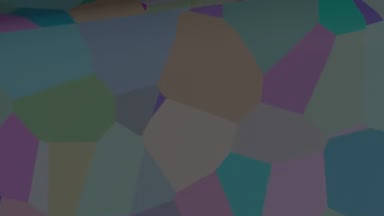
\includegraphics[width=\textwidth,height=0.5625\textheight]{docs/report/mfield/frame.jpg}
		\begin{axis}[title=Quiver and plot table,width=0.9\textwidth]
			\addplot[blue,quiver={u=\thisrow{u},v=\thisrow{v}},-stealth] table[col sep=comma] {docs/report/mfield/base.csv};
			\addplot[red,quiver={u=\thisrow{u},v=\thisrow{v}},-] table[col sep=comma] {docs/report/mfield/0.csv};
			\addplot[red,quiver={u=\thisrow{u},v=\thisrow{v}},-] table[col sep=comma] {docs/report/mfield/1.csv};
			\addplot[red,quiver={u=\thisrow{u},v=\thisrow{v}},-] table[col sep=comma] {docs/report/mfield/2.csv};
			\addplot[red,quiver={u=\thisrow{u},v=\thisrow{v}},-] table[col sep=comma] {docs/report/mfield/3.csv};
			\addplot[red,quiver={u=\thisrow{u},v=\thisrow{v}},-stealth] table[col sep=comma] {docs/report/mfield/4.csv};
			%{
			%	x y u v
			%	0 0 1 0
			%	0 	1 1 1 1
			%	0 	2 4 1 4
			%	0 	3 9 1 6
			%	0 	4 16 1 8
			%	0 };
			%\addplot[#3, mark = #4, thick, smooth, mark size = 2, mark options={fill=#3}] table [y=#2, col sep=comma] {\getstat{#1}};
		\end{axis}
	\end{tikzpicture}
	\caption{\centering Motionless gaps in the dense motion field. Colour of each bright dot represents direction of motion, while visible background area indicates lack of motion within the dense optical flow field.}
\end{figure}

\subsection{libmv estimator}

Blender's libmv library provides functions used by their built-in motion tracking tools\cite{blender-motion-tracking}. The tools are based on feature tracking and multiple view geometry reconstruction. The highest level class performing the estimation is EuclideanReconstruction, however, it requires points to be tracked throughout the scene. That is not possible to do online, due to frames into the future being unknown, and point tracking using optical flow not being particularly accurate, given discontinuities between motion vectors. The latter can be solved by pre-processing the motion vectors into a dense fixed-resolution structure and sampling motion vectors based on the pixel each vector lands on, however, that adds error and there still exists a risk of motionless gaps. Thus, we attempted to build our own estimation pipeline using lower level functions and the estimator crate was named libmv-estimator.

\begin{figure}[!ht]
	\centering
	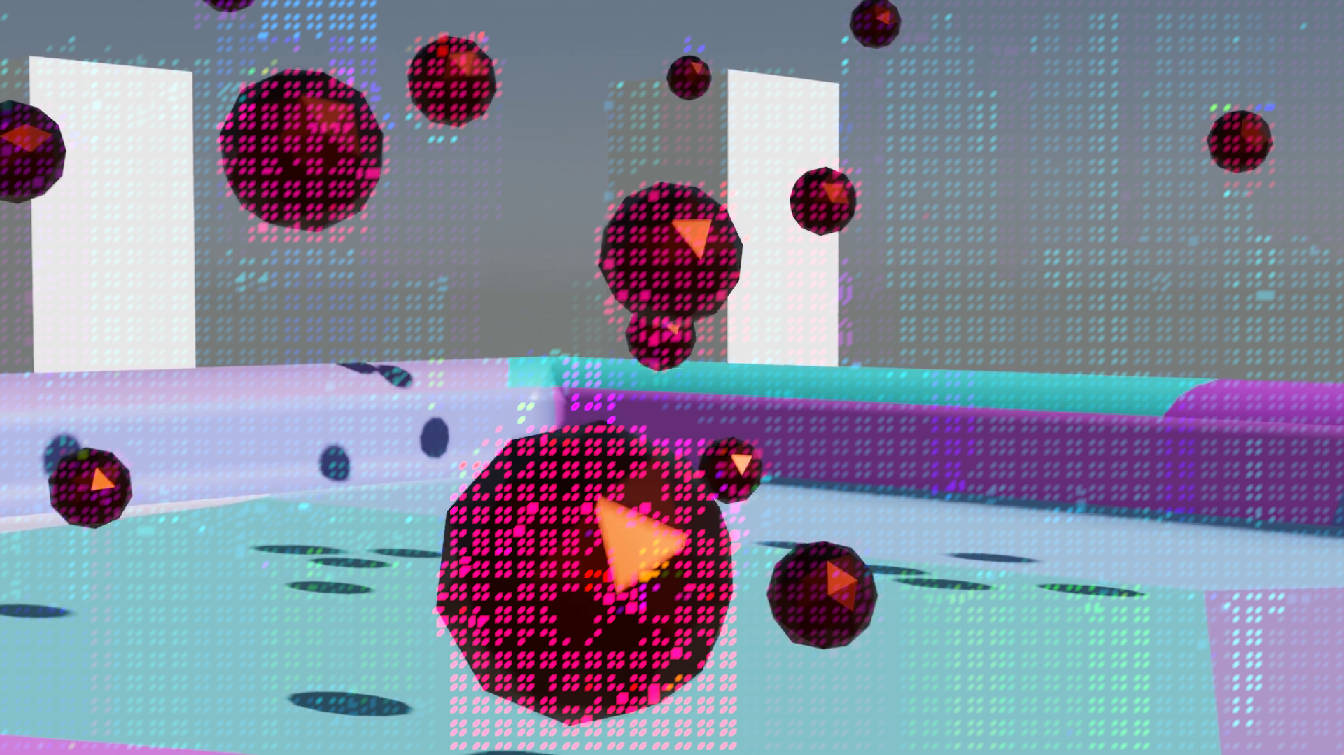
\includegraphics[width=250pt]{docs/report/mvec-gaps.jpg}
	\caption{\centering Motionless gaps in the dense motion field. Colour of each bright dot represents direction of motion, while visible background area indicates lack of motion within the dense optical flow field.}
\end{figure}

\subsubsection{Preparing libmv}

Several changes needed to be made to compile libmv, due to Fedora 35 packaging newer versions of libraries used by libmv, and they are available in commits fc7f41\footnote{fc7f41a484c3cb8df94e71b591076ab3c9e84827}-14ba45\footnote{14ba45e82847ff6bc98edad5abfd67c212328482} of our libmv fork\cite{libmv-fork}. The changes sum up to updating the APIs used in several third-party libraries, specifying typenames more correctly, and making changes in the CMake files to make the compilation work faster, and produce shared libraries out of the box. The fork has been added as a git submodule within libmv-rust directory.

Any C++ libraries need first to be wrapped in C ABI before used from Rust, due to C++ not having a stable ABI. Thus, libmv-rust crate was created. The crate contains a minimal set of functions used by the estimator. These functions were wrapped in C++ and re-exposed with C ABI. Finally, idiomatic Rust functions were created that allow easily calling into those wrappers.

\begin{figure}[!ht]
	\centering
	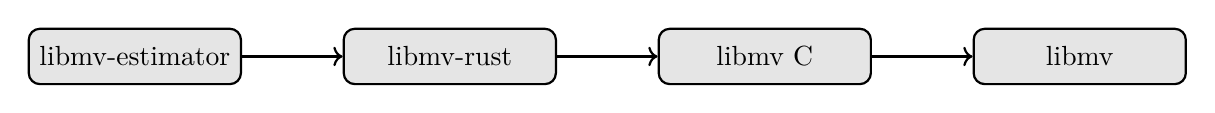
\begin{tikzpicture}
		[auto,
		block/.style ={rectangle, draw=black, thick, fill=black!10, text width=7em,align=center, rounded corners, minimum height=2em},
		line/.style ={draw, thick, -latex',shorten >=2pt},
		cloud/.style ={draw=red, thick, ellipse,fill=red!20,
		minimum height=1em}]
		\draw (0,0) node[block] (A) {libmv-estimator};
		\draw (4,0) node[block] (B) {libmv-rust};
		\draw (8,0) node[block] (C) {libmv C};
		\draw (12,0) node[block] (D) {libmv};
		\path[->, thick]
		(A)	edge node {} (B)
		(B) edge node {} (C)
		(C) edge node {} (D);

	\end{tikzpicture}
	\caption{\centering Flow of invoking libmv.}
\end{figure}

To use libmv-rust, location of compiled libmv libraries needs to be known. Thus, an environment file was created that can be sourced on linux using the source command.

\subsubsection{Pipeline}

Inside the pipeline we use either libmv's 7 or 8 point fundamental matrix estimation algorithm. The algorithm returns a fundamental matrix and a list of inlier motion vectors. This data is then used to compute essential matrix and its decomposition into camera motion. Upon correcting the scale of translation vector, relative pose change is returned.

\subsubsection{Triangulation}

Fundamental matrix resolves translational camera motion up to a scale factor, i.e. there is an implicit ambiguity\cite{hartley_zisserman_2004} of global translation: $\overrightarrow{t}_g = s\overrightarrow{t}$, where $\overrightarrow{t}$ is translation decomposed from $F$, and $s$ is the unknown scale factor. This ambiguity can not be resolved without more data - at least a third view is needed.

This paragraph introduces an algorithm for global scale triangulation. Assuming the camera is moving non-colinearly, current and previous motion vectors could be combined to build the relationship between 3 most recent views in the form of fundamental matrices $F_{12}$, $F_{23}$ and $F_{13}$. Decomposing the fundamental matrices we get 3 translation values $\overrightarrow{t}_{12}$, $\overrightarrow{t}_{23}$ and $\overrightarrow{t}_{13}$. In a noise-free environment, $s_{13}\overrightarrow{t}_{13} = \overrightarrow{t}_{g_{12}} + s_{23}\overrightarrow{t}_{23}$, where we assume that $\overrightarrow{t}_{g_{12}}$ is global translation of the previous frame. Solving $s_{23}$ by scaling it and $s_{13}$ until the equality matches allows us to compute a new vector $\overrightarrow{t}_{g_{23}} = s_{23}\overrightarrow{t}_{23}$, which is of consistent scale factor with $\overrightarrow{t}_{g_{12}}$. Continuing this process on the following frame is the same, except that $\overrightarrow{t}_{g_{23}}$ is now used as anchor for global scale.

\begin{figure}[!ht]
	\centering
	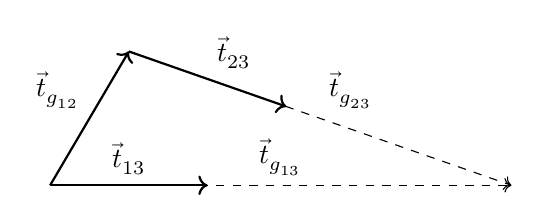
\begin{tikzpicture}
		[auto,
		block/.style ={rectangle, draw=black, thick, fill=black!10, text width=7em,align=center, rounded corners, minimum height=2em},
		line/.style ={draw, thick, -latex',shorten >=2pt},
		cloud/.style ={draw=red, thick, ellipse,fill=red!20,
		minimum height=1em}]
		\path[->, thick]
		(0,0) edge node {$\overrightarrow{t}_{g_{12}}$} (1,1.7)
		(1,1.7) edge node {$\overrightarrow{t}_{23}$} (3,1)
		(0,0) edge node {$\overrightarrow{t}_{13}$} (2,0);
		
		\path[->, dashed]
		(1,1.7) edge node {$\overrightarrow{t}_{g_{23}}$} (5.857,0)
		(0,0) edge node {$\overrightarrow{t}_{g_{13}}$} (5.857,0);

	\end{tikzpicture}
	\caption{\centering Triangulation. Local translation vectors are merely used as directions, while previous global translation vector can be used to resolve global scale of the new relative translations.}
\end{figure}

The main problem is accuracy. As stated earlier, tracking points with optical flow introduces error, thus accuracy of the relationship between the first and the third view is uncertain, and the translation vectors will not perfectly match. Inside our implementation we perform LU decomposition and solve for the scale factor that leads to a vector closest to the line defined by $\overrightarrow{t}_{13}$. However, if the camera moves colinearly, triangulation is not possible at all. Then, the points need to be tracked for more frames, which introduces further error and there is no reliable way to tell the scaling of the colinear view transforms. Thus, usability of this algorithm is uncertain.

\subsection{multiview estimator}

The following estimator is very similar to libmv-estimator. The crate is named multiview-estimator, and the key difference is that essential matrix is being computed instead of the fundamental one, which requires fewer data points. In addition, OpenCV library is being used, instead of libmv, which makes this estimator not require any custom build steps. The estimator suffers from the same translational scale problems and partial solution to that was discussed in the previous subsection. The properties system exposes 2 robust estimation modes of the estimator - RANSAC and LMedS\footnote{Lead Median of Squares}.

\subsection{homography estimator}

If two camera centers are coincident (there is no translational movement), all points in the view are related by homography\cite{hartley_zisserman_2004}, which is a type of matrix that relates coplanar points. Thus, assuming stationary camera we can use OpenCV's findHomography function to find the homography matrix and then decompose it to retrieve rotation information. homography-estimator crate implements this method.

\section{Motion detection}

Motion detection interface allows user to know whether there is motion in a scene or not. Optionally, it can provide regions of the scene with motion. We developed only one motion detector, its crate is named block-motion-detector and the next subsection describes its algorithm.

\subsection{Block motion detector}

As the name implies, this detector checks for motion in fixed size blocks. First, the algorithm filters out any insignificant motion vectors. A dense low resolution motion field is created where only motion vectors over the minimal motion magnitude threshold pass.

The next phase filters out noise and picks out motion that is of sufficiently large area by using Flood Fill algorithm. A block with sufficient motion is found and the algorithm checks all neighbors for motion. Any such neighbors get marked and then their neighbors get checked, so on until all connected blocks with motion get detected. This forms an island, and the algorithm finds the largest one.

If the resulting island has area over a certain thershold, the detector returns that there is motion, as well as the island itself. Parameters for minimal motion, target area, and motion field resolution are configurable by the user through the Properties trait. If configured correctly, the algorithm filters out noise and checks whether there is a moving object big enough to be considered for detection.

\begin{figure}[!ht]
	\centering
	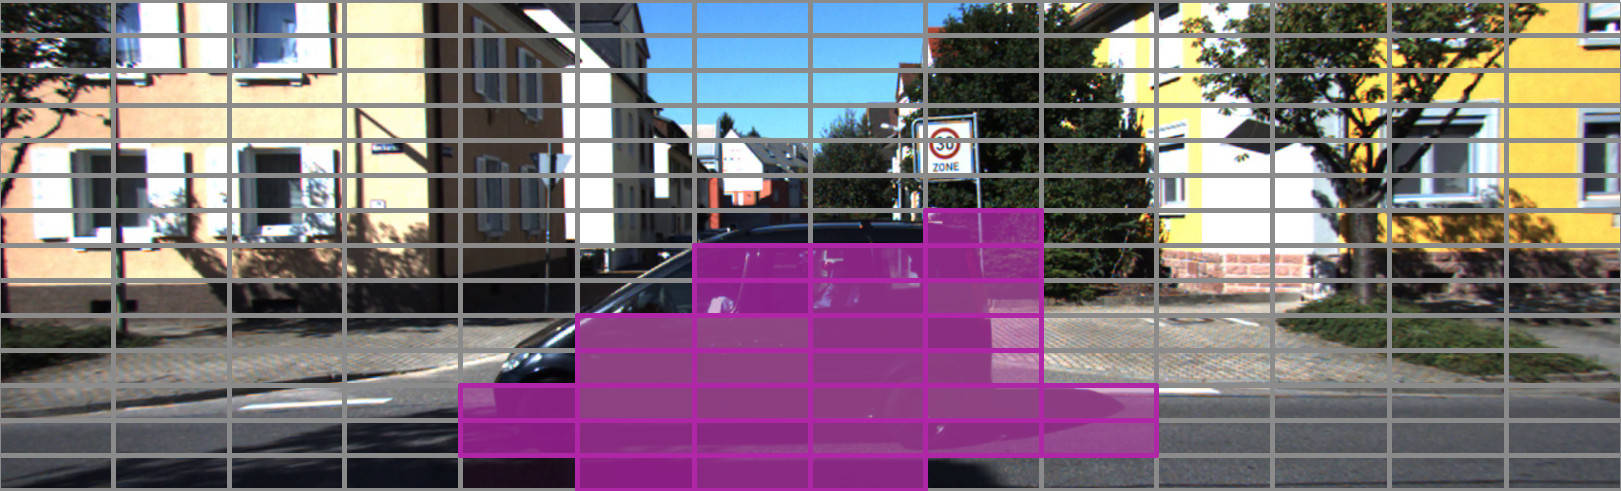
\includegraphics[width=350pt]{docs/report/detection.jpg}
	\caption{\centering Block motion detection. Grid indicates the resolution of detection motion field, and purple area shows the largest resulting island. The car in the image is driving to the left.}
\end{figure}

\section{OFPS Suite}

OFPS Suite is a graphical frontend for optical flow processing. The key design decision was to allow building in different optical flow processing applications with ease. At the top bar there is a list of apps, which can be extended in code by simply adding additional elements to an array of apps. This could also be trivially extended to dynamically load the applications up, but that was not necessary for our project.

\begin{figure}[!ht]
	\centering
	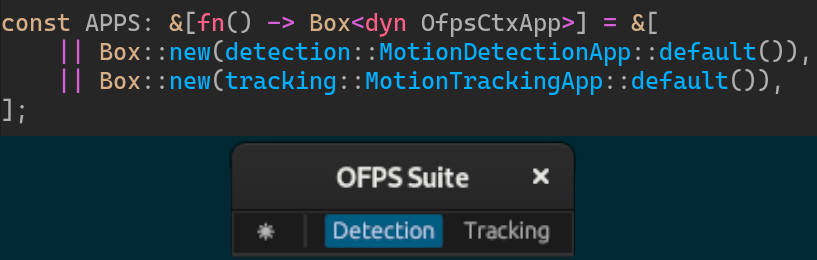
\includegraphics[width=250pt]{docs/report/ofps-suite-apps.jpg}
	\caption{\centering OFPS Suite applications in code.}
\end{figure}

We used egui\cite{egui} immediate mode UI framework, which is backend agnostic and works both on desktop, and in the web. This framework was chosen for its simplicity and integration with the rest of the Rust ecosystem. It can be rendered on top of other graphics, such as a 3D view, which is featured in the motion tracking tab.

Since dynamic OFPS plugin loading is at the heart of OFPS Suite, there is a single shared context that gets passed to the currently enabled app during render updates. The following subsections describe functionality and design of different OFPS Suite applications.

\subsection{Motion Detection}

Motion detection is the first application that was built for OFPS Suite. It provides the user a way to load up a video file or a stream using an arbitrary decoder, run motion detection using an arbitrary detector and then export timestamps of detection.

\subsubsection{Interface}

To perform motion detection, the user needs to load a decoder. List of available decoding plugins is available, as well as input for a video stream. By default, user is able to pick a file with a file dialog, but the widget can be toggled to allow for keyboard input, in cases such as TCP streams\footnote{To connect to a server at 192.168.0.92:3333, input tcp://192.168.0.92:3333}.

\textbf{Note:} the file dialog was built with rfd crate, and it was observed that at least in GNOME environments the dialog occasionally does not close. It appears to be an upstream issue, however, and not much can be done from our side.

Afterwards, the user needs to create a motion detection plugin. Similar structure is present in both of these widgets, because it was built in a modular way - the entire widget was defined by a trait that is implemented by each OFPS plugin type with minimal changes to suit their individual use case. 

By clicking the "Detection" button, menu options show up allowing the user to save and load parameters of the application in JSON format. The same file dialog widget is used as in decoder input.

Once both the decoder and the detector are created, video starts to be displayed. At the bottom of the window a timeline is visible displaying time regions with motion. On the left, additional information is available, such as the amount of motion in the frame as well motion vectors that correspond to dominant motion. There also is an ability to enable an overlay of detected motion and a button to export the timeline in CSV format.

It is possible to enable a performance summary and graph. The summary displays average performance of the decoder and the estimator, while the graph displays processing time at each individual frame. This data can then be exported in CSV format.

\subsubsection{Multithreaded Architecture}

Performing optical flow field decoding is a relatively intensive task and it would be detrimental to the user experience, if it was done on the main thread. Thus, the application was split into 2 threads - UI and worker. UI communicates with the worker thread - it accesses the latest results available and submits the latest state of runtime settings. Both of these variables are protected with a locking mechanism, but the worker accesses them only briefly to write the results and to read the latest settings. Overall, this architecture provides a smooth experience to the user, regardless of processing intensity in the worker thread.

\begin{figure}[!ht]
	\centering
	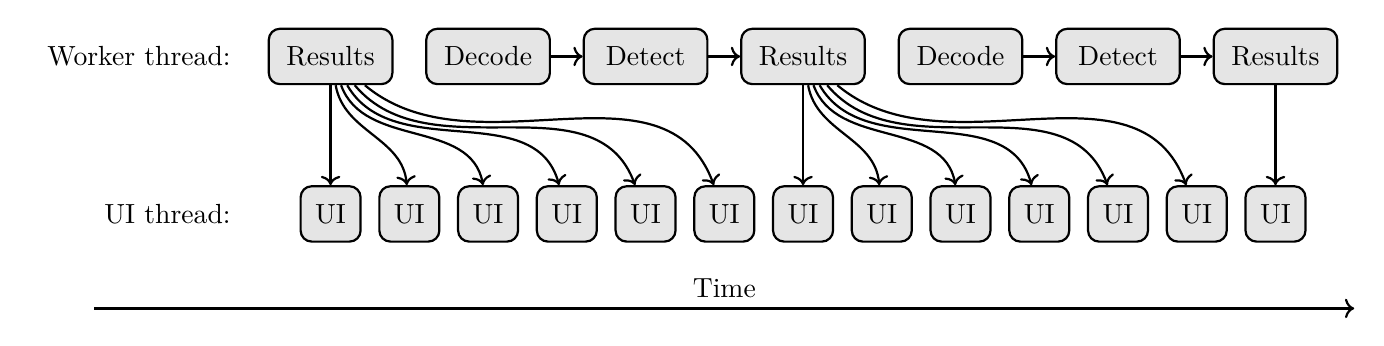
\begin{tikzpicture}
		[auto,
		block/.style ={rectangle, draw=black, thick, fill=black!10, text width=3.8em,align=center, rounded corners, minimum height=2em},
		line/.style ={draw, thick, -latex',shorten >=2pt},
		cloud/.style ={draw=red, thick, ellipse,fill=red!20,
		minimum height=1em},
		ui/.style = {block, text width=1.5em},
		nonrect/.style = {text width=7em,align=right, minimum height=2em},
		]
		
		\draw (-4.5,0) node[nonrect] (R1) {Worker thread:};
		\draw (-4.5,-2) node[nonrect] (R1) {UI thread:};

		\draw (-2,0) node[block] (R1) {Results};
		\draw (0,0) node[block] (DE1) {Decode};
		\draw (2,0) node[block] (DT1) {Detect};
		\draw (4,0) node[block] (R2) {Results};
		\draw (6,0) node[block] (DE2) {Decode};
		\draw (8,0) node[block] (DT2) {Detect};
		\draw (10,0) node[block] (R3) {Results};
		\draw (-2,-2) node[ui] (U0) {UI};
		\draw (-1,-2) node[ui] (U1) {UI};
		\draw (0,-2) node[ui] (U2) {UI};
		\draw (1,-2) node[ui] (U3) {UI};
		\draw (2,-2) node[ui] (U4) {UI};
		\draw (3,-2) node[ui] (U5) {UI};
		\draw (4,-2) node[ui] (U6) {UI};
		\draw (5,-2) node[ui] (U7) {UI};
		\draw (6,-2) node[ui] (U8) {UI};
		\draw (7,-2) node[ui] (U9) {UI};
		\draw (8,-2) node[ui] (U10) {UI};
		\draw (9,-2) node[ui] (U11) {UI};
		\draw (10,-2) node[ui] (U12) {UI};

		\path[->, thick, smooth]
		(DE1) edge node {} (DT1)
		(DT1) edge node {} (R2)
		(DE2) edge node {} (DT2)
		(DT2) edge node {} (R3)
		(R1) edge[out=270,in=90,->] node {} (U0)
		(R1) edge[out=280,in=95,->] node {} (U1)
		(R1) edge[out=290,in=100,->] node {} (U2)
		(R1) edge[out=300,in=105,->] node {} (U3)
		(R1) edge[out=310,in=110,->] node {} (U4)
		(R1) edge[out=320,in=110,->] node {} (U5)
		(R2) edge[out=270,in=90,->] node {} (U6)
		(R2) edge[out=280,in=95,->] node {} (U7)
		(R2) edge[out=290,in=100,->] node {} (U8)
		(R2) edge[out=300,in=105,->] node {} (U9)
		(R2) edge[out=310,in=110,->] node {} (U10)
		(R2) edge[out=320,in=110,->] node {} (U11)
		(R3) edge[out=270,in=90,->] node {} (U12);
		\path[->, thick]
		(-5,-3.2) edge node {Time} (11,-3.2);
	\end{tikzpicture}
	\caption{\centering Multithreaded architecture of motion detector.}
\end{figure}

\subsection{Motion Tracking}

Motion tracking is a more complex application that allows the user to create panoramas from video. It supports running multiple estimators simultaniously and also has built-in tools for comparing their estimates to ground-truth data.

\subsubsection{Interface}

Loading the decoder is done the same way as in the motion detection app, but it will start the decoding process immediately after creation. A few camera intrinsics need to be known for the estimation to work correctly, more specifically - vertical and horizontal fields of view. Any number of estimators may be added and each of them can be configured with general properties and ones specific to the estimator, such as accuracy parameters, used algorithm, etc. 3D view displays some of the estimated frames (it is possible to specify the number of frames drawn, however, too many of them may lead to out-of-memory scenarios). This view was built using a custom 3D renderer, which is described in the next section, and the camera can be orbitted around center of focus using the left mouse button, zoomed in and out with the scroll wheel, as well as panned with the mouse while holding the shift key.

\begin{figure}[!ht]
	\centering
	\centering
	\begin{subfigure}{230pt}
		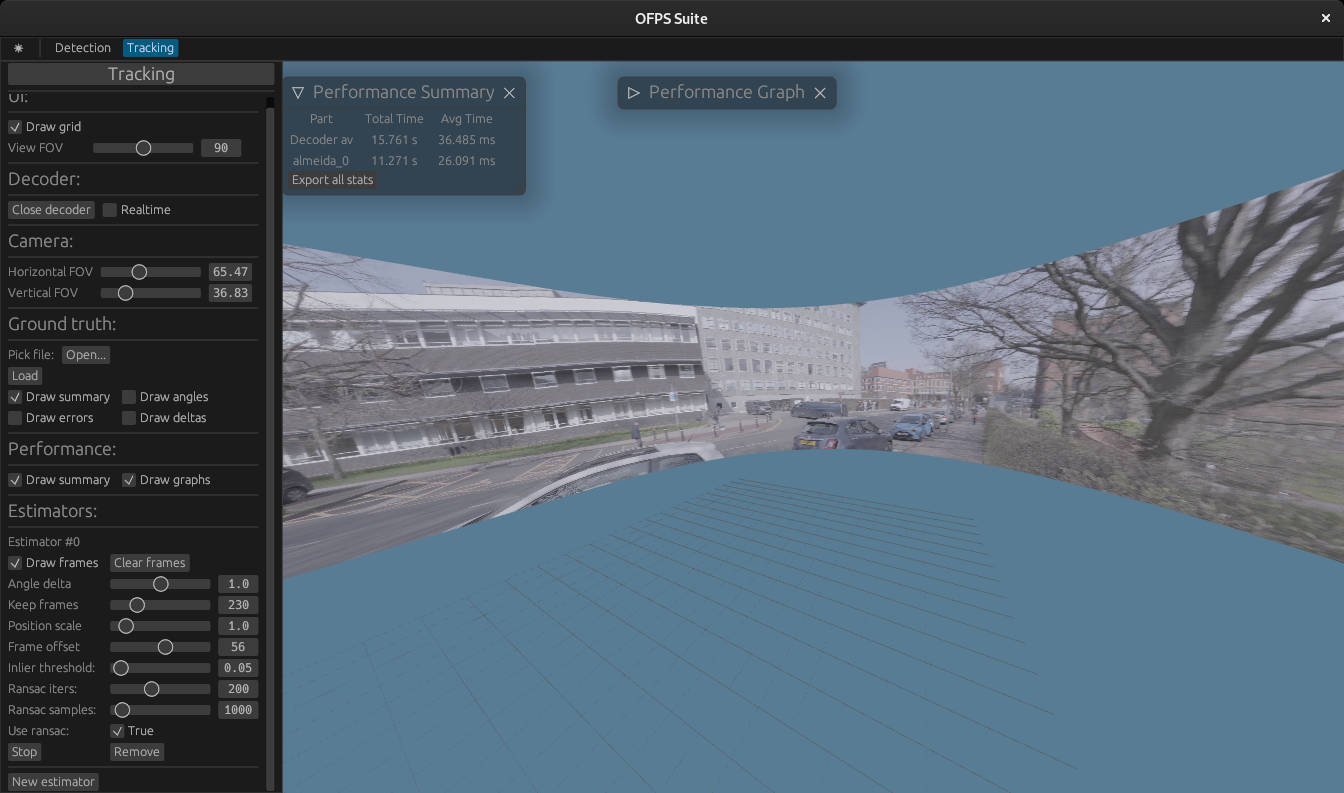
\includegraphics[width=230pt]{docs/report/panorama2.jpg}
	\end{subfigure}
	\begin{subfigure}{230pt}
		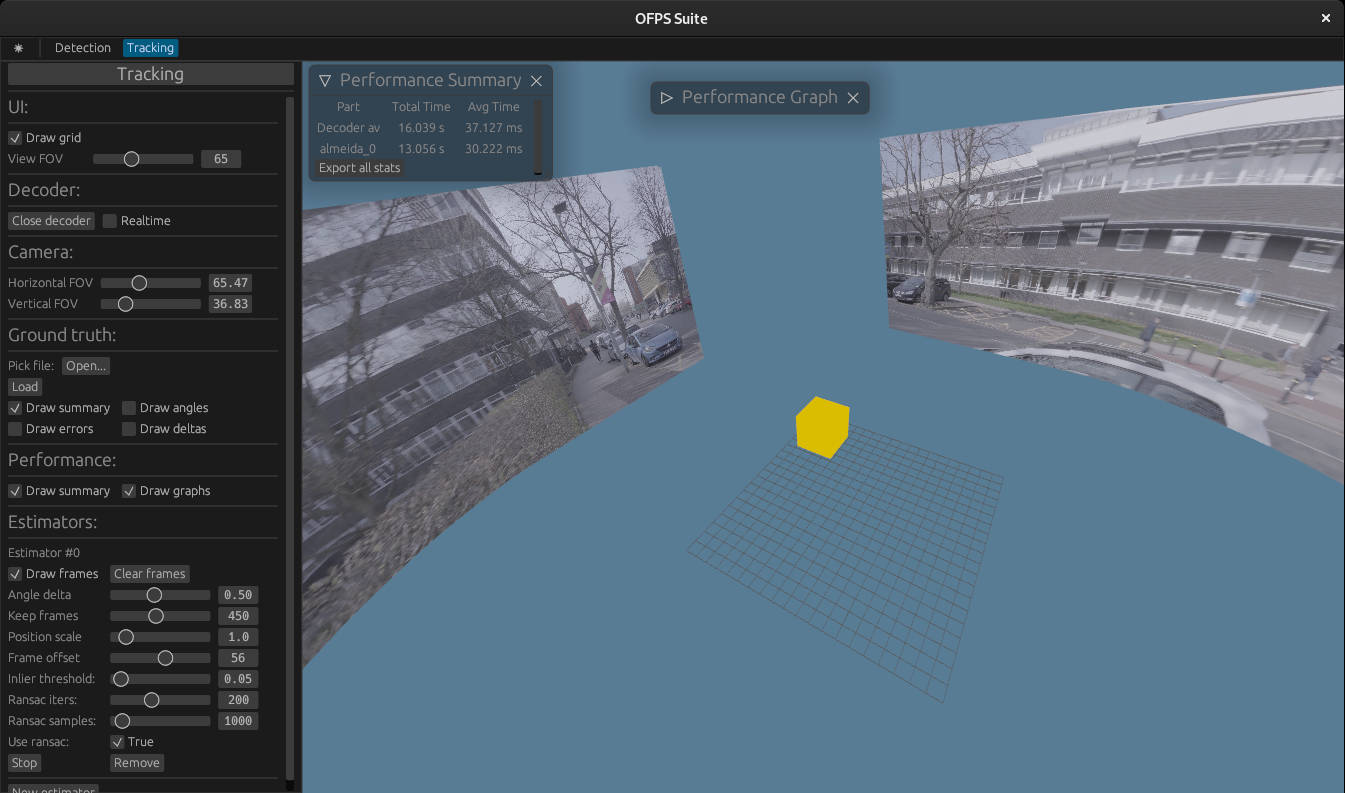
\includegraphics[width=230pt]{docs/report/panorama.jpg}
	\end{subfigure}
	\caption{\centering Panorama view. Yellow cube indicates the focus point around which the camera currently orbits around.}
\end{figure}

A ground truth CSV file may be loaded for comparison. Blender files for the project's synthetic videos use a script to export the truth data. Upon loading the data, average per-frame error of each estimator is computed and is shown in degrees. These results can then be exported, including indivudual per-frame errors and angles (in radians).

Similarly to the motion detection module, performance metrics are available. From the design standpoint, the exact same code is being run, thus providing streamlined user experience.

\subsubsection{Multithreaded Architecture}

Similar architecture to the one employed in motion detection app can also be found here. However, due to the details concerning frame transfer to GPU and performance implications of running multiple estimators, it is more complex.

When it comes to drawing frames, we are drawing multiple of them, instead of just the latest one, and worker thread can not load them itself on the GPU - all frames need to be sent to the UI thread first. Thus, there is a communication channel between the two threads where references to drawn frames get sent to the UI thread, which then loads raw RGBA data as a texture on GPU.

\begin{figure}[!ht]
	\centering
	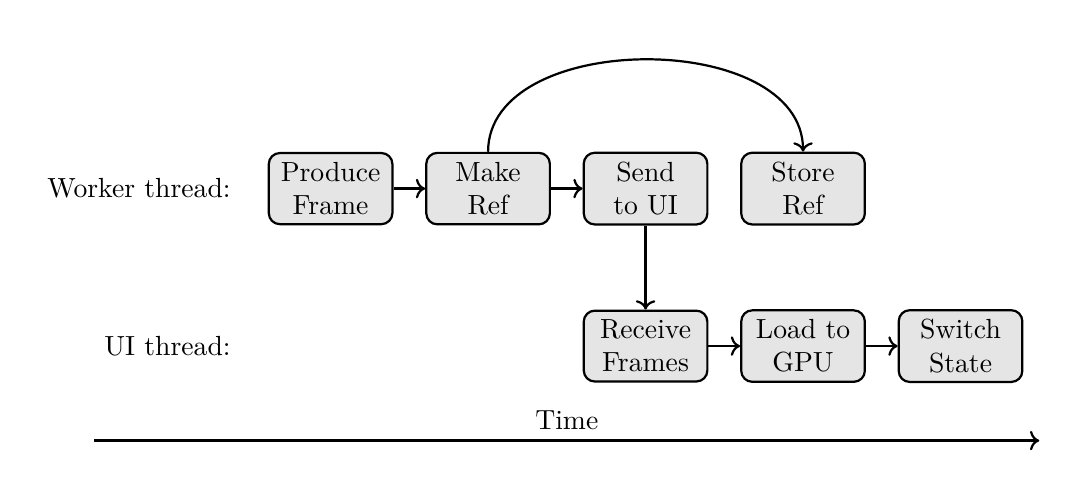
\begin{tikzpicture}
		[auto,
		block/.style ={rectangle, draw=black, thick, fill=black!10, text width=3.8em,align=center, rounded corners, minimum height=2em},
		line/.style ={draw, thick, -latex',shorten >=2pt},
		cloud/.style ={draw=red, thick, ellipse,fill=red!20,
		minimum height=1em},
		ui/.style = {block, text width=1.5em},
		nonrect/.style = {text width=7em,align=right, minimum height=2em},
		]
		
		\draw (-4.5,0) node[nonrect] (R1) {Worker thread:};
		\draw (-4.5,-2) node[nonrect] (R1) {UI thread:};

		\draw (-2,0) node[block] (R1) {Produce Frame};
		\draw (0,0) node[block] (R2) {Make Ref};
		\draw (2,0) node[block] (R3) {Send to UI};
		\draw (4,0) node[block] (R4) {Store Ref};
		\draw (2,-2) node[block] (U1) {Receive Frames};
		\draw (4,-2) node[block] (U2) {Load to GPU};
		\draw (6,-2) node[block] (U3) {Switch State};

		\path[->, thick, smooth]
		(R1) edge node {} (R2)
		(R2) edge node {} (R3)
		(R2) edge[out=90,in=90,->] node {} (R4)
		(R3) edge[out=270,in=90,->] node {} (U1)
		(U1) edge node {} (U2)
		(U2) edge node {} (U3);
		\path[->, thick]
		(-5,-3.2) edge node {Time} (7,-3.2);
	\end{tikzpicture}
	\caption{\centering Sequence of loading RGBA data on the GPU.}
\end{figure}

As for the estimators, they are being executed in parallel using rayon\cite{rayon}. However, motion estimation is a more complex task compared to simple boolean detection and the architecture would be suboptimal if decoding and estimation were to run in sequence. Thus, there is another worker thread dedicated to motion vector extraction - the thread decodes the optical flow field and sends the results out through a synchronised channel. The key detail here is that the channel is set up to be rendezvous\cite{rust_sync_channel} - the decoder thread blocks until the main worker thread is able to receive the results, thus only a single frame gets processed ahead of time. Upon accepting the result, worker thread executes the estimators, while the decoder thread performs motion vector extraction.

\begin{figure}[!ht]
	\centering
	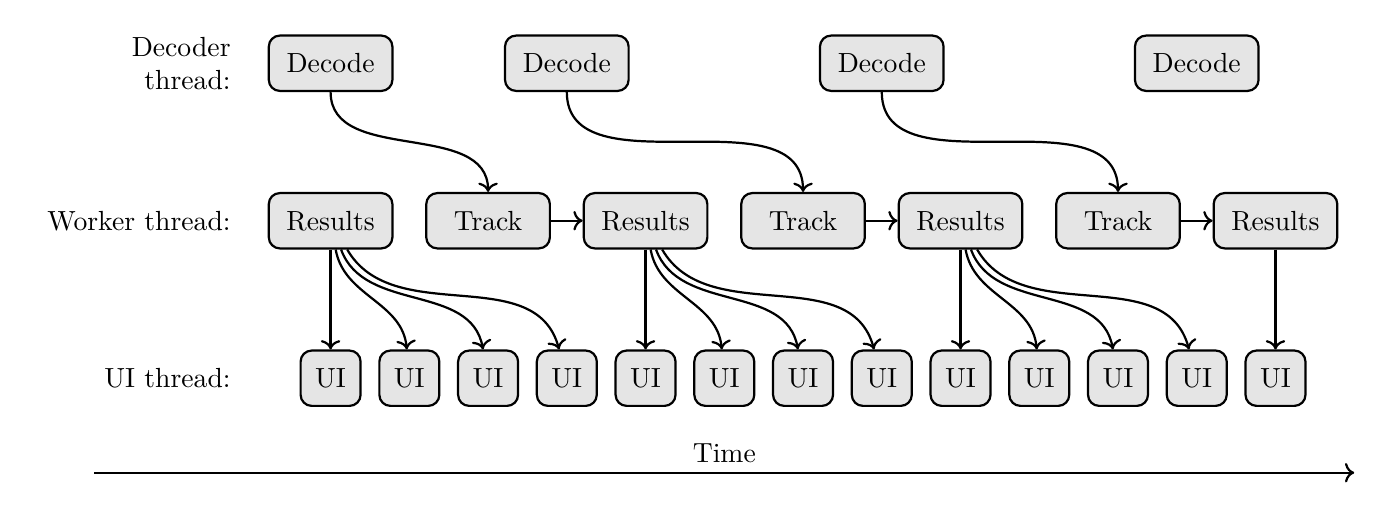
\begin{tikzpicture}
		[auto,
		block/.style ={rectangle, draw=black, thick, fill=black!10, text width=3.8em,align=center, rounded corners, minimum height=2em},
		line/.style ={draw, thick, -latex',shorten >=2pt},
		cloud/.style ={draw=red, thick, ellipse,fill=red!20,
		minimum height=1em},
		ui/.style = {block, text width=1.5em},
		nonrect/.style = {text width=7em,align=right, minimum height=2em},
		]
		
		\draw (-4.5,2) node[nonrect] (R1) {Decoder thread:};
		\draw (-4.5,0) node[nonrect] (R1) {Worker thread:};
		\draw (-4.5,-2) node[nonrect] (R1) {UI thread:};

		\draw (-2,0) node[block] (R1) {Results};
		\draw (-2,2) node[block] (DE1) {Decode};
		\draw (0,0) node[block] (DT1) {Track};
		\draw (2,0) node[block] (R2) {Results};
		\draw (1,2) node[block] (DE2) {Decode};
		\draw (4,0) node[block] (DT2) {Track};
		\draw (6,0) node[block] (R3) {Results};
		\draw (5,2) node[block] (DE3) {Decode};
		\draw (8,0) node[block] (DT3) {Track};
		\draw (10,0) node[block] (R4) {Results};
		\draw (9,2) node[block] (DE4) {Decode};
		\draw (-2,-2) node[ui] (U0) {UI};
		\draw (-1,-2) node[ui] (U1) {UI};
		\draw (0,-2) node[ui] (U2) {UI};
		\draw (1,-2) node[ui] (U3) {UI};
		\draw (2,-2) node[ui] (U4) {UI};
		\draw (3,-2) node[ui] (U5) {UI};
		\draw (4,-2) node[ui] (U6) {UI};
		\draw (5,-2) node[ui] (U7) {UI};
		\draw (6,-2) node[ui] (U8) {UI};
		\draw (7,-2) node[ui] (U9) {UI};
		\draw (8,-2) node[ui] (U10) {UI};
		\draw (9,-2) node[ui] (U11) {UI};
		\draw (10,-2) node[ui] (U12) {UI};

		\path[->, thick, smooth]
		(DE1) edge[out=270,in=90] node {} (DT1)
		(DT1) edge node {} (R2)
		(DE2) edge[out=270,in=90] node {} (DT2)
		(DT2) edge node {} (R3)
		(DE3) edge[out=270,in=90] node {} (DT3)
		(DT3) edge node {} (R4)
		(R1) edge[out=270,in=90,->] node {} (U0)
		(R1) edge[out=280,in=95,->] node {} (U1)
		(R1) edge[out=290,in=100,->] node {} (U2)
		(R1) edge[out=300,in=105,->] node {} (U3)
		(R2) edge[out=270,in=90,->] node {} (U4)
		(R2) edge[out=280,in=95,->] node {} (U5)
		(R2) edge[out=290,in=100,->] node {} (U6)
		(R2) edge[out=300,in=105,->] node {} (U7)
		(R3) edge[out=270,in=90,->] node {} (U8)
		(R3) edge[out=280,in=95,->] node {} (U9)
		(R3) edge[out=290,in=100,->] node {} (U10)
		(R3) edge[out=300,in=105,->] node {} (U11)
		(R4) edge[out=270,in=90,->] node {} (U12);
		\path[->, thick]
		(-5,-3.2) edge node {Time} (11,-3.2);

	\end{tikzpicture}
	\caption{\centering Multithreaded architecture of motion tracking app. Tracking steps are further split in parallel using rayon parallel for\_each loops.}
\end{figure}

\section{wimrend 3D renderer}

wimrend crate was built as a standalone 3D renderer for our OFPS Suite app. While it was designed for the purposes of OFPS motion tracking visualisation, general usage was considered to make the architecture modular, flexible and otherwise tidy. wimrend uses wgpu crate for lower level graphics API calls. wgpu is a mid-level abstraction of WebGPU - a rendering and computation API for the web browsers\cite{webgpu}. However, since WebGPU is an incomplete standard, wgpu currently implements a number of different backends, such as Vulkan, OpenGL, Metal, WebGL, Direct3D 11 and 12, while keeping the same mid-level API for setting up GPU buffers, render passes, issuing draw calls etc. Thus, wgpu was a clear choice for us, due to its portability and fine-grained control of the rendering process.

\subsection{Renderer API}

A minimal API was designed for drawing 3D objects on the scene in immediate mode. There is a function for drawing a mesh with custom material, colour and 3D pose onto screen. The renderer handles lower level details, such as loading meshes and materials on the GPU, writing pose and colour information into the instance buffer\footnote{A buffer that stores minimal set of properties that differ between individual objects}. The user only needs to add objects to render each frame, and set up scene parameters, such as camera view and background colour. There also exists a function for 3D line rendering - these lines can be occluded by objects, as they are rendered on the same render pass.

All materials, textures and meshes are being stored in deduplicated reference counted manner. If a material is no longer used, its shaders will be unloaded from the GPU, if a texture is not being used, its buffer will be freed as well. The only current limitation is with meshes - the mesh manager does not track whether a mesh is used or not and it does not get unloaded until the program exits. However, this can only become a problem when an object with constantly changing geometry is being drawn, and OFPS Suite does not do that. Reloading meshes comes at a performance penalty, thus it was decided against doing it.

\subsection{Performance}

GPUs are parallel processing devices that incur heavy latency in sequential calls, thus one of the biggest bottlenecks in older graphics engines is the number of draw calls being issued. Modern rendering engines solve this by using a technique called instancing. Recent graphics APIs provide a way to draw a list of identical meshes using slightly different per-instance parameters, hence the name instancing. Given a list of objects our renderer partitions the objects in a way that minimises the number of draw calls being issued. Each instanced batch depends on the rendering pipeline being used (shaders of the material), textures being bound, and the mesh. The final per-instance parameters, such as object's transformation matrix and colour are then being provided as a list in a single instanced draw call.

\subsection{Additional rendering}

The previous subsections only described the process of drawing 3D objects onto the scene, however, user interface needs to be drawn as well. This is done in the form of additional render passes. Once 3D objects are drawn, egui, or other rendering engine can layer their drawing operations on top. This is enabled through the RenderSubState trait. The trait accepts input, pre-render and on-render events which allow to drive custom app logic and perform custom rendering operations. OFPS suite makes use of this trait to draw its GUI on top.

\begin{figure}[!ht]
	\centering
	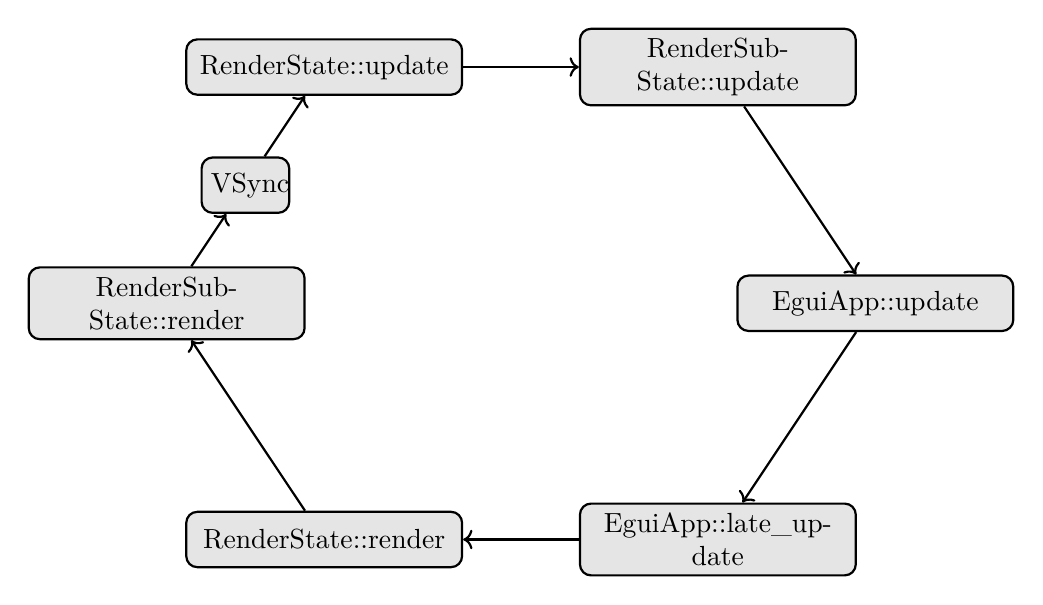
\begin{tikzpicture}
		[auto,
		block/.style ={rectangle, draw=black, thick, fill=black!10, text width=9.3em,align=center, rounded corners, minimum height=2em},
		line/.style ={draw, thick, -latex',shorten >=2pt},
		cloud/.style ={draw=red, thick, ellipse,fill=red!20,
		minimum height=1em},
		ui/.style = {block, text width=2.5em},
		nonrect/.style = {text width=7em,align=right, minimum height=2em},
		]
		
		\draw (-2.5,0) node[block] (R1) {RenderState::update};
		\draw (2.5,0) node[block] (R2) {RenderSubState::update};
		\draw (4.5,-3) node[block] (R3) {EguiApp::update};
		\draw (2.5,-6) node[block] (R4) {EguiApp::late\_update};
		\draw (-2.5,-6) node[block] (R5) {RenderState::render};
		\draw (-4.5,-3) node[block] (R6) {RenderSubState::render};
		\draw (-3.5,-1.5) node[ui] (R7) {VSync};

		\path[->, thick, smooth]
		(R1) edge node {} (R2)
		(R2) edge node {} (R3)
		(R3) edge node {} (R4)
		(R4) edge node {} (R5)
		(R5) edge node {} (R6)
		(R6) edge node {} (R7)
		(R7) edge node {} (R1);

	\end{tikzpicture}
	\caption{\centering Render loop with OFPS Suite's substate.}
\end{figure}


\chapter{Results}

In this section we present end results of the project. Effectiveness of the motion detection is evaluated, estimators are compared against ground truth data, and modularity of OFPS is evaluated. Functionality of OFPS Suite has been omitted, since it has already been detailed in methods.

\section{Detection}

In order to test motion detection effectiveness, we placed the Raspberry Pi with the camera to look outside a room and recorded 30 minutes worth of raw H.264 packets. A scenario was set up to imitate burglary: 7 minutes into the video home owner leaves and walks past the camera, a few minutes later thief walks into the house, walking past the camera. 17 minutes later the thief leaves the house and a few minutes later the home owner comes back. Our motion detection system was able to successfully identify all of those cases and not emit any false positives. Numerous small tests were also performed, and given correct parameter configuration, the system was robust.

\section{Estimation}

In order to test the estimators a large number of tests were conducted using different video files, optical flow computation methods, and estimator configurations. This section briefly explains the configuration and evaluates results collected in those configurations.

In total, 192 comparisons were made. 8 estimator configurations were compared - 2 per each estimator type. 8 different 3D rendered videos were created in Blender, and performance of each estimator was compared against the ground truth data extracted from the camera's animation. All clips performed the exact same motions, in the given sequence: panning, tilting, combined panning and tilting, rolling, and all 3 axis combined. The only difference between the clips is the environment - there are 4 different backgrounds of decreasing level of detail, which should lead to less accurate optical flows, and each of them has a static and dynamic version. Dynamic version adds moving spheres and the idea behind that was to test how well each estimator deals with presence of outliers. Multiple runs of estimation were performed using 3 different optical flow generation methods: MPEG, Farneback and RLOF (both at fixed 150x84 resolution). We picked such low resolution, because epipolar geometry based estimators could not handle that many motion vectors.

We attempted to track translational movement of the camera as well, but the performance of libmv and multiview estimators was unsuitable for analysis. Even using prior knowlege of the video to normalise estimated translation vectors did not yield accurate results. Thus, we decided against testing that.

\begin{figure}[!ht]
	\centering
	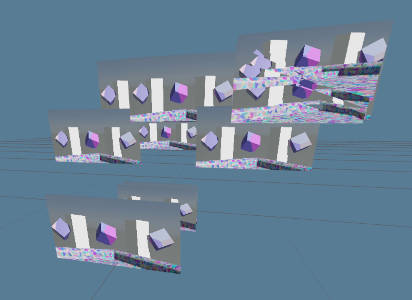
\includegraphics[width=150pt]{docs/report/translation.jpg}
	\caption{\centering Noisy translation estimation with libmv estimator.}
\end{figure}

\subsection{Runtime Performance}

Figure below plots average performance of each estimator under different optical flow decoders. These results have been averaged over all 8 sample videos. Due to large differences in processing time across estimators, these results are plotted in logaritmic scale, however, the overall trend of the runtime performance is rather clear. Almeida and homography estimators are reasonably lightweight in most conditions, and can easily handle over 10000 motion vectors produced by OpenCV based decoders each frame. However, epipolar geometry based estimators are not able to handle that many data points, thus, their runtime performance suffers. In all cases, the fastest estimator is Homography-RANSAC. Almeida and Homography based estimators are able to process at least 30 frames per second, while epipolar geometry based estimators are not usable at all in realtime scenarios. Let us see now how accurate the results are.

\begin{figure}[!ht]
\begin{center}
\begin{tikzpicture}
	\begin{axis}[
			xlabel = {Decoder},
			ylabel = {Processing time (ms per frame)},
			ymode = log,
			ymax = 100000,
			ytick={1,10,16.7,33.3,100,1000,10000},
			yticklabels={1,10,16.7,33.3,100,1000,10000},
			symbolic x coords={av,rlof,farneback},
			xtick={av,farneback,rlof},
			xticklabels={MPEG,Farneback,RLOF},
			width = \textwidth,
			height = 0.5\textwidth,
			legend cell align=left,
			legend columns=2,
			legend pos = north west
		]
		\legend{
			30 FPS Threshold, 60 FPS Threshold,
			Almeida-RANSAC,Almeida,
			Homography-RANSAC,Homography-LMedS,
			Multiview-RANSAC,Multiview-LMedS,
			Libmv-7pt,Libmv-8pt,
		}
		\addplot[magenta, thick, dotted] table {
			av 33.333
			av 33.333
			farneback 33.333
		};
		\addplot[green, thick, dotted] table {
			av 16.666
			av 16.666
			farneback 16.666
		};
		\statplot{perf.csv}{Almeida-RANSAC}{teal}{*};
		\statplot{perf.csv}{Almeida}{teal}{o, dashed};
		\statplot{perf.csv}{Homography-RANSAC}{blue}{*};
		\statplot{perf.csv}{Homography-LMedS}{blue}{o, dashed};
		\statplot{perf.csv}{Multiview-RANSAC}{red}{*};
		\statplot{perf.csv}{Multiview-LMedS}{red}{o, dashed};
		\statplot{perf.csv}{Libmv-7pt}{orange}{*};
		\statplot{perf.csv}{Libmv-8pt}{orange}{o, dashed};
	\end{axis}
\end{tikzpicture}
\end{center}
\caption{\centering Estimator runtime performance comparison under different optical flow decoders.}
\end{figure}

\subsection{Accuracy}

The next few graphs compare average accuracy of the estimator in different environments. The lower the average error the better. Comparing estimator accuracy with MPEG motion vectors (see figure 4.2) we can see that by far the most accurate estimator is our modified implementation of the method proposed by Almeida et al. Specifically, RANSAC version performs exceptionally well. Only in the fourth environment does it start to loose to the least-squares configuration. Almeida-RANSAC is able to successfully eliminate any outliers that non-RANSAC version uses for model fitting. Curiously, Almeida-RANSAC seems to perform marginally better in dynamic environments than static ones. This could be attributed to the video encoder being forced to transform background macroblocks more in line with the true motion in presence of other moving objects. The same anomaly can be found in multiview and 7 point libmv estimators. Speaking of other estimators, RANSAC configurations appear to perform better than LMedS based ones, and 8 point fundamental matrix based algorithm struggles to perform accurate predictions, especially in dynamic environments. Overall, Almeida-RANSAC is the best performing estimator in this case.

\begin{figure}[!ht]
\begin{center}
\begin{tikzpicture}
	\begin{axis}[
			xlabel = {Video clip},
			ylabel = {Average error (degrees)},
			ymax = 0.35,
			symbolic x coords={1,1dyn,2,2dyn,3,3dyn,4,4dyn},
			xtick={1,1dyn,2,2dyn,3,3dyn,4,4dyn},
			xticklabels = {
				\vidpic{vid1.jpg},
				\vidpic{vid1dyn.jpg},
				\vidpic{vid2.jpg},
				\vidpic{vid2dyn.jpg},
				\vidpic{vid3.jpg},
				\vidpic{vid3dyn.jpg},
				\vidpic{vid4.jpg},
				\vidpic{vid4dyn.jpg},
			},
			every axis x label/.style={
				at={(0.5,-0.2)},
				anchor=center,
			},
			width = \textwidth,
			height = 0.5\textwidth,
			legend cell align=left,
			legend columns=2,
			legend pos = north west
		]
		\legend{
			Almeida-RANSAC,Almeida,
			Homography-RANSAC,Homography-LMedS,
			Multiview-RANSAC,Multiview-LMedS,
			Libmv-7pt,Libmv-8pt
		}
		\statplot{err_av.csv}{Almeida-RANSAC}{teal}{*};
		\statplot{err_av.csv}{Almeida}{teal}{o, dashed};
		\statplot{err_av.csv}{Homography-RANSAC}{blue}{*};
		\statplot{err_av.csv}{Homography-LMedS}{blue}{o, dashed};
		\statplot{err_av.csv}{Multiview-RANSAC}{red}{*};
		\statplot{err_av.csv}{Multiview-LMedS}{red}{o, dashed};
		\statplot{err_av.csv}{Libmv-7pt}{orange}{*};
		\statplot{err_av.csv}{Libmv-8pt}{orange}{o, dashed};
	\end{axis}
\end{tikzpicture}
\end{center}
\caption{\centering Estimator performance comparison on encoded H.264 streams.}
\end{figure}

Figure 4.3 shows very similar relative performance when using OpenCV's base Gunnar-Farneback implementation. However, the overall accuracy seems to degrade from the third environment, and the results from all estimators seem to be very similar, which could indicate that this decoder was unable to produce accurate enough optical flows.

\begin{figure}[!ht]
\begin{center}
\begin{tikzpicture}
	\begin{axis}[
			xlabel = {Video clip},
			ylabel = {Average error (degrees)},
			ymax = 0.4,
			symbolic x coords={1,1dyn,2,2dyn,3,3dyn,4,4dyn},
			xtick={1,1dyn,2,2dyn,3,3dyn,4,4dyn},
			xticklabels = {
				\vidpic{vid1.jpg},
				\vidpic{vid1dyn.jpg},
				\vidpic{vid2.jpg},
				\vidpic{vid2dyn.jpg},
				\vidpic{vid3.jpg},
				\vidpic{vid3dyn.jpg},
				\vidpic{vid4.jpg},
				\vidpic{vid4dyn.jpg},
			},
			every axis x label/.style={
				at={(0.5,-0.2)},
				anchor=center,
			},
			width = \textwidth,
			height = 0.5\textwidth,
			legend cell align=left,
			legend columns=2,
			legend pos = north west
		]
		\legend{
			Almeida-RANSAC,Almeida,
			Homography-RANSAC,Homography-LMedS,
			Multiview-RANSAC,Multiview-LMedS,
			Libmv-7pt,Libmv-8pt
		}
		\statplot{err_farneback.csv}{Almeida-RANSAC}{teal}{*};
		\statplot{err_farneback.csv}{Almeida}{teal}{o, dashed};
		\statplot{err_farneback.csv}{Homography-RANSAC}{blue}{*};
		\statplot{err_farneback.csv}{Homography-LMedS}{blue}{o, dashed};
		\statplot{err_farneback.csv}{Multiview-RANSAC}{red}{*};
		\statplot{err_farneback.csv}{Multiview-LMedS}{red}{o, dashed};
		\statplot{err_farneback.csv}{Libmv-7pt}{orange}{*};
		\statplot{err_farneback.csv}{Libmv-8pt}{orange}{o, dashed};
	\end{axis}
\end{tikzpicture}
\end{center}
\caption{\centering Estimator performance comparison using optical flows computed with Gunnar-Farneback algorithm.}
\end{figure}

Optical flows produced by RLOF appear to have consistent quality throughout the clips, and the results are relatively similar to the ones observed using MPEG motion vectors. In figure 4.5, we can notice that Libmv-8pt consistently performs the worst, which is consistent with results of processing Farneback optical flows.

\begin{figure}
\begin{center}
\begin{tikzpicture}
	\begin{axis}[
			xlabel = {Video clip},
			ylabel = {Average error (degrees)},
			ymax = 0.4,
			symbolic x coords={1,1dyn,2,2dyn,3,3dyn,4,4dyn},
			xtick={1,1dyn,2,2dyn,3,3dyn,4,4dyn},
			xticklabels = {
				\vidpic{vid1.jpg},
				\vidpic{vid1dyn.jpg},
				\vidpic{vid2.jpg},
				\vidpic{vid2dyn.jpg},
				\vidpic{vid3.jpg},
				\vidpic{vid3dyn.jpg},
				\vidpic{vid4.jpg},
				\vidpic{vid4dyn.jpg},
			},
			every axis x label/.style={
				at={(0.5,-0.2)},
				anchor=center,
			},
			width = \textwidth,
			height = 0.5\textwidth,
			legend cell align=left,
			legend columns=2,
			legend pos = north west
		]
		\legend{
			Almeida-RANSAC,Almeida,
			Homography-RANSAC,Homography-LMedS,
			Multiview-RANSAC,Multiview-LMedS,
			Libmv-7pt,Libmv-8pt
		}
		\statplot{err_rlof.csv}{Almeida-RANSAC}{teal}{*};
		\statplot{err_rlof.csv}{Almeida}{teal}{o, dashed};
		\statplot{err_rlof.csv}{Homography-RANSAC}{blue}{*};
		\statplot{err_rlof.csv}{Homography-LMedS}{blue}{o, dashed};
		\statplot{err_rlof.csv}{Multiview-RANSAC}{red}{*};
		\statplot{err_rlof.csv}{Multiview-LMedS}{red}{o, dashed};
		\statplot{err_rlof.csv}{Libmv-7pt}{orange}{*};
		\statplot{err_rlof.csv}{Libmv-8pt}{orange}{o, dashed};
	\end{axis}
\end{tikzpicture}
\end{center}
\caption{\centering Estimator performance comparison using optical flows computed with RLOF.}
\end{figure}

Given Almeida-RANSAC is the most accurate estimator, figure 4.4 compares the performance of it under different optical flow generation methods. In there we can notice how well MPEG holds up in higher contrast scenarios - Almeida-RANSAC performs nearly identically in the first 3 environments under MPEG compression to RLOF. Only the 4th scene leads to divergence in accuracy, however, real-world videos rarely contain this little detail, so it remains to be seen how well the estimator performs there. Farneback decoder appears to enable more accurate estimation in the second environment, however, its optical flow appears to diverge from reality in lower complexity environments.

\begin{figure}[!ht]
\begin{center}
\begin{tikzpicture}
	\begin{axis}[
			xlabel = {Video clip},
			ylabel = {Average error (degrees)},
			symbolic x coords={1,1dyn,2,2dyn,3,3dyn,4,4dyn},
			xtick={1,1dyn,2,2dyn,3,3dyn,4,4dyn},
			xticklabels = {
				\vidpic{vid1.jpg},
				\vidpic{vid1dyn.jpg},
				\vidpic{vid2.jpg},
				\vidpic{vid2dyn.jpg},
				\vidpic{vid3.jpg},
				\vidpic{vid3dyn.jpg},
				\vidpic{vid4.jpg},
				\vidpic{vid4dyn.jpg},
			},
			every axis x label/.style={
				at={(0.5,-0.3)},
				anchor=center,
			},
			width = \textwidth,
			height = 0.4\textwidth,
			legend cell align=left,
			legend columns=2,
			legend pos = north west
		]
		\legend{
			MPEG,
			RLOF,
			Farneback
		}
		\statplot{err_av.csv}{Almeida-RANSAC}{teal}{*};
		\statplot{err_rlof.csv}{Almeida-RANSAC}{red}{*};
		\statplot{err_farneback.csv}{Almeida-RANSAC}{orange}{*};
	\end{axis}
\end{tikzpicture}
\end{center}
\caption{\centering Almeida-RANSAC estimator compared with optical flow calculation methods.}
\end{figure}

\pagebreak

\subsection{Real-world data}

The leading estimator was tested against real world clips as well, where a stationary camera pans around the scene. Modified almeida estimator is able to accurately track camera motion and panorama view gets created (see figure 3.9).

\section{OFPS}

Optical Flow Processing Stack can be evaluated by its modularity. The core library consists of a thousand lines of code, which is reused by the plugin crates. Each plugin averages around 300 lines of code and only concerns itself with providing functionality with minimal boilerplate code.

(Figure: code size)

From the user's perspective, the API is concise and the following code can be used to perform motion estimation:

\begin{minted}[numbersep=5pt,frame=lines,framesep=2mm,linenos]{rust}
let store = PluginStore::new();

let mut decoder = store.create_decoder("av", "input.mp4".into())?;
let mut estimator = store.create_estimator("almeida", Default::default())?;

let mut mv = vec![];
let mut pos = Default::default();
let mut rot = Default::default();

while let Ok(_) = decoder.process_frame(&mut mv, None, 0) {
    estimator.motion_step(&mv, camera, None, &mut rot, &mut pos)?;
    println!("{pos:?} | {:?}", rot.euler_angles());
}
\end{minted}

\chapter{Conclusion}

This project showed that MPEG motion vectors are robust in motion detection tasks and that stationary camera motion tracking is viable with motion estimators that were built specifically for resolving 3 degrees of rotation freedom. We were also able to conclude that position of the camera is not trackable using conventional multiple view geometry based methods due to MPEG vectors being too noisy for the task. A modular library was built enabling simple a path to building different optical flow calculation methods, motion estimators and detectors. A sophisticated application was built on top of the stack enabling any user to perform motion detection and estimation tasks. A 3D renderer was designed from scratch to aid visualising the results.

\section{Discussion and Future Work}

Overall, while the project did not validate all hypotheses, it achieved its main goals of building a modular optical flow processing stack and with it, building applications of MPEG motion vector processing. However, there are several improvements that could be done, given more time.

Firstly, it would have been great to test sparse optical flow methods, such as the Lucas-Kanade method\cite{lucas-kanade}. It was observed that MPEG motion vectors enabled to achieve good results while being relatively sparse. Thus, testing out this proven sparse optical flow method may be beneficial.

It would also be very interesting to see just how fast motion vector extraction is using a custom H.264 stream decoder that does not perform any frame reconstruction. We observed that libav is able to process individual packets very fast, however, the decoding step was the most intensive.

In addition, it would be interesting to look at other video encoding standards. High Efficiency Video Coding, also known as H.265 or MPEG-H Part 2, was published in 2013, and contains a lot of changes compared to previous standards. For starters, the I-frames are using a new image format, known as High Efficiency Image Format, or HEIF in short. Furthermore, HEVC does not use fixed size macroblocks - it instead uses Coding Tree Units (CTUs) that vary in size between $16 \times 16$ and $64 \times 64$ pixels\cite{h265}. While AVC is only able to represent 8 directions of motion, HEVC transform blocks can move in 31 different directions. Thus, HEVC has the potential to contain more accurate motion information and it would be interesting to write a custom decoding module for H.265 streams. Furthermore, we did not look at any video encoders designed by AOM\footnote{Alliance for Open Media}, such as AV1, which contains more complex prediction features, such as global motion compensation\cite{av1}\cite{av1_global_motion}, and it would be beneficial to conduct further research, given the first AV1 encoding capable graphics cards have recently been made available.

We were unable to track camera's translational motion using optical flow methods. Given more time, we could have attempted to develop a more robust solution. One possible solution would be to compute the trifocal tensor\cite{hartley_zisserman_2004}. Another way would be to reconstruct 3D position of the inliers and attempt aligning them with the previous frame, which is a very similar approach to the one employed by VOLDOR, however, it is still uncertain whether any of these solutions would work.

It was very surprising to see how well the modified Almeida estimator performed, compared to other proven methods. Building a model that does not go beyond the constraints imposed by the problem appears to be highly beneficial, and while other estimators have more degrees of freedom, their accuracy suffers in simpler cases. In addition, estimation being more accurate in presence of outliers surprised us even more. We inspected the motion vectors of 2 final video files in ffplay\footnote{Run "ffplay -flags2 e+export\_mvs -vf codecview=mv=pf+bb <input\_video>"} and were able to notice the dynamic version encoding motion in a more complex manner, while the static version would often take shortcuts and encode the exact same motion in low contrast areas as the one present in the white pillars above them. Finally, the modularity of our optical flow processing stack opens possibilities to conduct further research in this field with less friction.

\printbibliography

\end{document}
